\chapter{Listado de primitivas}
   \label{Listado-Primitivas}
   \index{Listado de primitivas}

Como dec\'iamos, la tortuga se controla por medio de comandos internos
llamados \textit{primitivas}. Las siguientes secciones definen estas
primitivas:

\section{Movimientos de la tortuga; poner l\'apiz y colores}
   \label{Movimientos-Colores}

\subsection{Movimientos}
   \label{Movimientos}

Esta primera tabla define las primitivas que gobiernan el movimiento
de la tortuga, y s\'olo necesitan un argumento:
\begin{center}
 \begin{longtable}{*{2}{|m{3cm}}|m{9cm}|} \hline
   \multicolumn{1}{|c|}{\textbf{Primitivas}} & 
      \multicolumn{1}{c|}{\textbf{Argumentos}} &
         \multicolumn{1}{c|}{\textbf{Uso}} \\ \endhead \hline 
   \texttt{avanza}, \index{avanza@\texttt{avanza}}
     \texttt{av} \index{av@\texttt{av}} & \texttt{n: n\'umero de pasos} &
          Mueve la tortuga hacia adelante \texttt{n} pasos en la
          direcci\'on que actualmente est\'a mirando. \\ \hline 
   \texttt{retrocede}, \index{retrocede@\texttt{retrocede}}
     \texttt{re} \index{re@\texttt{re}} & \texttt{n: n\'umero de pasos} &
          Mueve la tortuga hacia atr\'as \texttt{n} pasos en la direcci\'on
          que actualmente est\'a mirando. \\ \hline 
   \texttt{giraderecha}, \index{giraderecha@\texttt{giraderecha}}
     \texttt{gd} \index{gd@\texttt{gd}} & \texttt{n: \'angulo} &
          Gira la tortuga \texttt{n} grados hacia la derecha de la direcci\'on
          que actualmente est\'a mirando. \\ \hline 
   \texttt{giraizquierda}, \index{giraizquierda@\texttt{giraizquierda}}
     \texttt{gi} \index{gi@\texttt{gi}} & \texttt{n: \'angulo} &
          Gira la tortuga \texttt{n} grados hacia la izquierda de la
          direcci\'on que actualmente est\'a mirando. \\ \hline 
\end{longtable} \end{center}

En esta segunda tabla el movimiento se controla mediante \textbf{coordenadas} en
la pantalla. Para ver mejor dichas coordenadas, se dispone de las primitivas
\texttt{cuadr\'icula}, que muestra una cuadr\'icula en pantalla de las dimensiones
deseadas, y \texttt{ejes}, que muestra los ejes cartesianos con las correspondientes 
etiquetas: 
\begin{center}
 \begin{longtable}{|m{3.5cm}|m{3cm}|m{8.5cm}|} \hline
   \multicolumn{1}{|c|}{\textbf{Primitivas}} & 
      \multicolumn{1}{c|}{\textbf{Argumentos}} &
         \multicolumn{1}{c|}{\textbf{Uso}} \\ \endhead \hline
   \texttt{cuadr\'icula} \index{cuadr\'icula@\texttt{cuadr\'icula}} &
      \texttt{a b: n\'umeros} &
        Dibuja una cuadr\'icula en el \textbf{\'Area de dibujo} de dimensiones 
         \texttt{a} x \texttt{b} y borra la pantalla\\ \hline
   \texttt{borracuadr\'icula}\index{borracuadr\'icula@\texttt{borracuadr\'icula}}
%   \texttt{detienecuadr\'icula}\index{detienecuadr\'icula@\texttt{detienecuadr\'icula}}
      & \texttt{no} &
        Quita la cuadr\'icula del \textbf{\'Area de dibujo} y borra la pantalla
          \\ \hline
 \texttt{poncolorcuadr\'icula}\index{poncolorcuadr\'icula@\texttt{poncolorcuadr\'icula}}
      \texttt{pcc}\index{pcc@\texttt{pcc}} &
      \texttt{primitiva}, \texttt{lista} o \texttt{numero} &
        Establece el color de la cuadr\'icula del \textbf{\'Area de dibujo}
          \\ \hline
   \texttt{colorcuadr\'icula}\index{colorcuadr\'icula@\texttt{colorcuadr\'icula}} & 
      \texttt{no} &
        Devuelve el color actual de la cuadr\'icula. \\ \hline
   \texttt{ejes}\index{ejes@\texttt{ejes}}&
      \texttt{a: n\'umero}  &
        Dibuja los ejes cartesianos (X e Y) de escala (separaci\'on entre marcas)
        \texttt{a}, con las etiquetas correspondientes.
          \\ \hline
   \texttt{ejex}\index{ejex@\texttt{ejex}}&
      \texttt{a: n\'umero}  &
        Dibuja el eje de abscisas (eje X) de escala (separaci\'on entre marcas)
        \texttt{a}, con las etiquetas correspondientes.
          \\ \hline
   \texttt{ejey}\index{ejey@\texttt{ejey}}&
      \texttt{a: n\'umero}  &
        Dibuja el eje de ordenadas (eje Y) de escala (separaci\'on entre marcas)
        \texttt{a}, con las etiquetas correspondientes.
          \\ \hline
   \texttt{borraejes}\index{borraejes@\texttt{borraejes}}
%   \texttt{detieneejes}\index{detieneejes@\texttt{detieneejes}}
      & \texttt{no}  &
        Quita los ejes del \textbf{\'Area de dibujo} y borra la pantalla
            \\ \hline
   \texttt{poncolorejes}\index{poncolorejes@\texttt{poncolorejes}}
      \texttt{pce}\index{pce@\texttt{pce}} &
      \texttt{primitiva}, \texttt{lista} o \texttt{numero} &
        Establece el color de los ejes en el \textbf{\'Area de dibujo}
            \\ \hline
   \texttt{colorejes}\index{colorejes@\texttt{colorejes}} &
      \texttt{no} &
        Devuelve el color actual de los ejes. \\ \hline \hline
   \texttt{centro} \index{centro@\texttt{centro}} & \texttt{no} &
          Lleva la tortuga a la posici\'on original, es decir coordenadas
          \texttt{[0 0]} con rumbo \texttt{0}. \\ \hline 
   \texttt{posici\'on}, \index{posici\'on@\texttt{posici\'on}} 
      \texttt{pos} \index{pos@\texttt{pos}} & \texttt{no} &
        Devuelve las coordenadas X e Y de la posici\'on actual
        de la tortuga.\\ \hline 
   \texttt{ponposici\'on}, \index{ponposici\'on@\texttt{ponposici\'on}}
     \texttt{ponpos} \index{ponpos@\texttt{ponpos}} &
        \texttt{[x y]: lista de dos n\'umeros}&
          Mueve la tortuga a las coordenadas especificadas por los dos
          n\'umeros en la lista (\texttt{x} es la abscisa, \texttt{y} la
          ordenada). \\ \hline 
   \texttt{ponx} \index{ponx@\texttt{ponx}} & \texttt{x: eje x} &
          Mueve la tortuga horizontalmente hasta el punto de abscisa \texttt{x}
                 \\ \hline 
   \texttt{pony} \index{pony@\texttt{pony}} & \texttt{y: eje y} &
          Mueve la tortuga verticalmente hasta el punto de ordenada \texttt{y}
                  \\ \hline 
   \texttt{ponxy} \index{ponxy@\texttt{ponxy}} & 
       \texttt{x y}: coordenadas \texttt{x} e \texttt{y} &
          Id\'entico a \texttt{ponpos [x y]} \texttt{x} e \texttt{y} son
          n\'umeros, no una lista. \\ \hline 
   \texttt{punto} \index{punto@\texttt{punto}} & \texttt{a: lista} &
          El punto definido por las coordenadas de la lista se resaltar\'a
          con el color del l\'apiz. \\ \hline
\end{longtable} \end{center}

Esta tercera tabla muestra las primitivas que controlan el rumbo, direcci\'on
en grados respecto de la vertical y mirando hacia arriba:
\begin{center}
 \begin{longtable}{*{2}{|m{3cm}}|m{9cm}|} \hline
   \multicolumn{1}{|c|}{\textbf{Primitivas}} & 
      \multicolumn{1}{c|}{\textbf{Argumentos}} &
         \multicolumn{1}{c|}{\textbf{Uso}} \\ \endhead \hline
   \texttt{rumbo} \index{rumbo@\texttt{rumbo}} & \texttt{no} &
        Devuelve el rumbo o el \'angulo de la tortuga.\\ \hline 
   \texttt{ponrumbo}, \index{ponrumbo@\texttt{ponrumbo}} 
     \texttt{ponr} \index{ponr@\texttt{ponr}} & \texttt{n: rumbo} &
          Orienta la tortuga en la direcci\'on especificada. \texttt{0}
          corresponde a mirar hacia arriba verticalmente. \\ \hline 
   \texttt{hacia} \index{hacia@\texttt{hacia}} & \texttt{a: lista} &
        La lista debe contener dos n\'umeros que representen coordenadas.
        Devuelve el rumbo que la tortuga deber\'a seguir hacia el punto
        definido por las coordenadas.\\ \hline 
   \texttt{distancia} \index{distancia@\texttt{distancia}} & 
      \texttt{a: lista} &
        La lista debe contener dos n\'umeros que representen coordenadas.
        Devuelve el n\'umero de pasos desde la actual posici\'on y el punto
        definido por las coordenadas.\\ \hline 
\end{longtable} \end{center}

\subsection{Propiedades}
   \label{Propiedades-Tortuga}
   \index{Propiedades}

Esta tabla descrine las primitivas que permiten ajustar las propiedades de la
tortuga. Por ejemplo, ?`estar\'a visible en la pantalla? ?`Con qu\'e color
dibujar\'a cuando se mueva?

\begin{center} \begin{longtable}{*{2}{|m{3cm}}|m{9cm}|} \hline  
    \multicolumn{1}{|c|}{\textbf{Primitivas}} &
       \multicolumn{1}{c|}{\textbf{Argumentos}} &
          \multicolumn{1}{c|}{\textbf{Uso}} \\ \endhead \hline 
   \texttt{muestratortuga}, \index{muestratortuga@\texttt{muestratortuga}}
     \texttt{mt} \index{mt@\texttt{mt}} & \texttt{no} &
        Hace que la tortuga se vea en pantalla. \\ \hline 
   \texttt{ocultatortuga}, \index{ocultatortuga@\texttt{ocultatortuga}}
     \texttt{ot} \index{ot@\texttt{ot}} & \texttt{no} &
        Hace invisible a la tortuga. \\ \hline 
   \texttt{bajal\'apiz}, \index{bajal\'apiz@\texttt{bajal\'apiz}}
     \texttt{bl} \index{bl@\texttt{bl}} & \texttt{no} &
        La tortuga dibujar\'a una l\'inea cuando se mueva. \\ \hline 
   \texttt{subel\'apiz}, \index{subel\'apiz@\texttt{subel\'apiz}}
     \texttt{sl} \index{sl@\texttt{sl}} & \texttt{no} &
        La tortuga no dibujar\'a cuando se mueva. \\ \hline 
   \texttt{goma}, \index{goma@\texttt{goma}}
     \texttt{go} \index{go@\texttt{go}} & \texttt{no} &
        La tortuga borrar\'a toda traza que encuentre.\\ \hline 
   \texttt{inviertel\'apiz}, \index{inviertel\'apiz@\texttt{inviertel\'apiz}}
     \texttt{ila} \index{ila@\texttt{ila}} & \texttt{no} &
        Pone la tortuga en ``modo inverso'', y l\'apiz abajo.
              \\ \hline 
   \texttt{ponl\'apiz}, \index{ponl\'apiz@\texttt{ponl\'apiz}}
     \texttt{pla} \index{pla@\texttt{pla}} & \texttt{no} &
        Pone la tortuga en el modo normal de dibujo y l\'apiz abajo. \\ \hline 
   \texttt{poncolorl\'apiz}, \index{poncolorl\'apiz@\texttt{poncolorl\'apiz}}
     \texttt{poncl} \index{poncl@\texttt{poncl}} & 
        \texttt{a: n\'umero, primitiva o lista [r v a]} &
           Cambia el color del l\'apiz.
           La especificaci\'on del color se detalla en la secci\'on
            \ref{AcercaColores} \\ \hline 
   \texttt{pongrosor} \index{pongrosor@\texttt{pongrosor}} & 
      \texttt{n: n\'umero} &
        Define el grosor del trazo del l\'apiz (en pixels). Por defecto es 1.
        La forma es cuadrada.\\ \hline 
   \texttt{colorl\'apiz}, \index{colorl\'apiz@\texttt{colorl\'apiz}}
     \texttt{cl} \index{cl@\texttt{cl}} & \texttt{a: lista} &
        Devuelve el color actual del l\'apiz. \\ \hline 
   \texttt{encuentracolor}, \index{encuentracolor@\texttt{encuentracolor}}
     \texttt{ec} \index{ec@\texttt{ec}} & \texttt{a: lista} &
        Devuelve el color del punto definido por las coordenadas. \\ \hline
   \texttt{grosorl\'apiz}, \index{grosorl\'apiz@\texttt{grosorl\'apiz}}
   \texttt{gl} \index{gl@\texttt{gl}} & \texttt{no} &
        Devuelve el grosor del l\'apiz. \\ \hline 
   \texttt{ponformal\'apiz}, \index{ponformal\'apiz@\texttt{ponformal\'apiz}}
   \texttt{pfl} \index{pfl@\texttt{pfl}} & \texttt{n: 0 \'o 1} &
        Fija la forma del l\'apiz: \texttt{pfl 0}: cuadrada; 
        \texttt{pfl 1}: ovalada. \\ \hline 
   \texttt{formal\'apiz}, \index{formal\'apiz@\texttt{formal\'apiz}}
   \texttt{fl} \index{fl@\texttt{fl}} & \texttt{no} &
        Devuelve la forma del l\'apiz. \\ \hline 
   \texttt{ponforma}, \index{ponforma@\texttt{ponforma}} 
      \texttt{pforma} \index{pforma@\texttt{pforma}} & \texttt{n: n\'umero} &
        Puedes elegir tu tortuga preferida en la segunda etiqueta del men\'u
        \textbf{Herramientas $\rightarrow$ Preferencias}, pero tambi\'en es posible
        con \texttt{ponforma}. El n\'umero \texttt{n} puede ir de 0 a 6. (0 es 
        la forma triangular del \textsc{Logo} tradicional). \\ \hline 
   \texttt{forma} \index{forma@\texttt{forma}} & \texttt{no} &
        Devuelve un n\'umero que representa la forma actual de la tortuga.
           \\ \hline 
\end{longtable} \end{center}

El control del \'Area de dibujo se realiza con las primitivas siguientes:
\begin{center} \begin{longtable}{|m{3.5cm}|m{3cm}|m{8.5cm}|} \hline  
    \multicolumn{1}{|c|}{\textbf{Primitivas}} &
       \multicolumn{1}{c|}{\textbf{Argumentos}} &
          \multicolumn{1}{c|}{\textbf{Uso}} \\ \endhead \hline 
   \texttt{poncolorpapel}, \index{poncolorpapel@\texttt{poncolorpapel}}
     \texttt{poncp} \index{poncp@\texttt{poncp}} & 
        \texttt{a: n\'umero, primitiva o lista [r v a]} &
           Cambia el color del papel (fondo).
           La especificaci\'on del color se detalla en la secci\'on
            \ref{AcercaColores} \\ \hline 
   \texttt{colorpapel} \index{colorpapel@\texttt{colorpapel}} &
     \texttt{a: lista} &
        Devuelve el color actual del ``papel'' (fondo, \'area
        de dibujo). \\ \hline 
   \texttt{poncalidaddibujo}, \index{poncalidaddibujo@\texttt{poncalidaddibujo}} 
   \texttt{pcd} \index{pcd@\texttt{pcd}}  & \texttt{n: 0, 1 \'o 2} &
        Fija la calidad del dibujo: \texttt{pcd 0}: normal;
         \texttt{pcd 1}: alta; \texttt{pcd 2}: baja; \\ \hline  
   \texttt{calidaddibujo}, \index{calidaddibujo@\texttt{calidaddibujo}}
   \texttt{cdib} \index{cdib@\texttt{cdib}} & \texttt{no} &
        Devuelve la calidad del dibujo \\ \hline 
   \texttt{tama\~nopantalla}, \index{tama\~nopantalla@\texttt{tama\~nopantalla}}
   \texttt{tpant} \index{tpant@\texttt{tpant}} & \texttt{no} &
        Devuelve una lista que contiene el tama\~no de la pantalla \\ \hline 
   \texttt{pontama\~nopantalla}
       \index{pontama\~nopantalla@\texttt{pontama\~nopantalla}}
   \texttt{ptp} \index{@ptp\texttt{ptp}} & \texttt{a: lista} &
        Fija el tama\~no de la pantalla. Ejemplo: \texttt{ptp [1000 1000]} \\ \hline
   \texttt{modoventana} \index{modoventana@\texttt{modoventana}} &
      \texttt{no} &
        La tortuga puede salir del \'area de dibujo (pero no dibujar\'a nada).
           \\ \hline 
   \texttt{modovuelta} \index{modovuelta@\texttt{modovuelta}} & \texttt{no} &
        Si la tortuga sale del \'area de dibujo, vuelve a aparecer en el lado
        opuesto \\ \hline 
   \texttt{modojaula} \index{modojaula@\texttt{modojaula}} & \texttt{no} &
        La tortuga queda confinada al \'area de dibujo. Si intenta salir,
        aparecer\'a un mensaje de error avisando cu\'antos pasos faltan
        para el punto de salida. \\ \hline 
   \texttt{tama\~noventana}, \index{tama\~noventana@\texttt{tama\~noventana}} 
     \texttt{tv}, \index{tv@\texttt{tv}}
   \texttt{esquinasventana} \index{esquinasventana@\texttt{esquinasventana}} &
      \texttt{no} &
        Devuelve una lista con cuatro elementos, las coordenadas de la esquina
        superior izquierda y de la esquina inferior derecha.

        Por ejemplo, si devuelve \texttt{[-200 200 400 -300]}, significa que
        las coordenadas de la esquina superior izquierda son \texttt{(-200,200)}
        y las de la esquina inferior derecha \texttt{(400,-300)}\\ \hline 
   \texttt{zoom} \index{zoom@\texttt{zoom}} &
      \texttt{a: n\'umero} &
        Acerca o aleja el \'Area de dibujo. En concreto, el valor de \texttt{a}
        es el factor de escala respecto a la imagen original:
        \texttt{(a>1)} acerca el \'Area de dibujo;  
        \texttt{(0<a<1)} aleja el \'Area de dibujo. \\ \hline
   \texttt{borrapantalla}, \index{borrapantalla@\texttt{borrapantalla}}
     \texttt{bp} \index{bp@\texttt{bp}} & \texttt{no} &
        Vac\'ia el \'area de dibujo, situando a la tortuga en el centro de
        la pantalla. \\ \hline 
   \texttt{limpia} \index{limpia@\texttt{limpia}} & \texttt{no} &
        Vac\'ia el \'area de dibujo, dejando a la tortuga en el lugar donde
        estaba tras la ejecuci\'on anterior.\\ \hline 
\end{longtable} \end{center}

Finalmente, las primitivas que controlan la escritura en pantalla, los mensajes
al usuario y simplifican determinados dibujos:
\begin{center} \begin{longtable}{*{2}{|m{3cm}}|m{9cm}|} \hline  
    \multicolumn{1}{|c|}{\textbf{Primitivas}} &
       \multicolumn{1}{c|}{\textbf{Argumentos}} &
          \multicolumn{1}{c|}{\textbf{Uso}} \\ \endhead \hline 
   \texttt{rotula} \index{rotula@\texttt{rotula}} & 
       \texttt{a: palabra o lista} & 
          Dibuja la palabra o lista especificada, en la posici\'on actual,
          y en la direcci\'on que est\'a mirando. \\ \hline 
   \texttt{largoetiqueta}
       \index{largoetiqueta@\texttt{largoetiqueta}} & \texttt{a: lista} &
          Devuelve, en p\'ixels, la longitud que tendr\'a en pantalla la
          lista. \\ \hline
   \texttt{ponfuente}, \index{ponfuente@\texttt{ponfuente}}
     \texttt{pf} \index{pf@\texttt{pf}} & \texttt{n: n\'umero} &
        Cuando se escribe con la primitiva \texttt{rotula}, modifica el tama\~no
        de la tipograf\'ia. Por defecto, el tama\~no es 12. \\ \hline 
   \texttt{fuente} \index{fuente@\texttt{fuente}} & \texttt{no} &
        Devuelve el tama\~no de la tipograf\'ia cuando se escribe en pantalla
        con la primitiva rotula. \\ \hline 
   \texttt{mensaje}, \index{mensaje@\texttt{mensaje}}
     \texttt{msj}\index{msj@\texttt{msj}} & \texttt{a: lista} &
        Muestra una caja de di\'alogo con el mensaje que est\'a en la lista.
        El programa se detiene hasta que el usuario hace un \textit{click} en
        el bot\'on ``Aceptar'' \\ \hline
   \texttt{c\'irculo} \index{c\'irculo@\texttt{c\'irculo}} & \texttt{n: radio} &
          Dibuja una circunferencia de radio \texttt{n} alrededor de la
          tortuga \\ \hline 
   \texttt{arco} \index{arco@\texttt{arco}} & \texttt{n: radio}
                                                \texttt{a~b:~\'angulos} &
          Dibuja un arco de circunferencia de radio \texttt{n} alrededor
          de la tortuga, comprendido entre los \'angulos \texttt{a} y
          \texttt{b}, midiendo desde el rumbo de la tortuga. \\ \hline 
\end{longtable}\end{center}

La primitiva \texttt{largoetiqueta} permite saber si al escribir en
pantalla con \texttt{rotula} tienes suficiente espacio.
\begin{quote}
   \noindent \textbf{Ejemplo}:

   \texttt{largoetiqueta [Hola, ?`c\'omo est\'as?]} devuelve, en p\'ixels
   la longitud en pantalla de la frase \textit{Hola, ?`c\'omo est\'as?} 
\end{quote}

\subsection{La tortuga en Tres Dimensiones}
   \label{3-Dimensiones}
   \index{3d} \index{Tres Dimensiones}

Desde la versi\'on 0.9.92, nuestra tortuga puede dejar el plano para trasladarse
a un espacio en tres dimensiones (3D). Para cambiar a esta modalidad,
Usaremos la primitiva \texttt{perspectiva}. !`Bienvenido a un mundo en 3D!
\index{perspectiva@\texttt{perspectiva}}

Para recuperar el modo bidimensional (2D), debemos indicarle que vuelva a uno
de los modos ``planos'': \texttt{modojaula}, \texttt{modoventana} o 
\texttt{modovuelta}. \index{modojaula@\texttt{modojaula}}
\index{modovuelta@\texttt{modovuelta}}\index{modoventana@\texttt{modoventana}}

\subsubsection{La proyecci\'on en perspectiva}

Para representar un espacio 3D en un plano 2D, \textsc{Xlogo} utiliza una
proyecci\'on en perspectiva. Es equivalente a tener una c\'amara grabando
la escena en 3D, y mostrando en la pantalla la imagen de la proyecci\'on.
Veamos un esquema gr\'afico para explicarlo mejor:
\begin{center}
   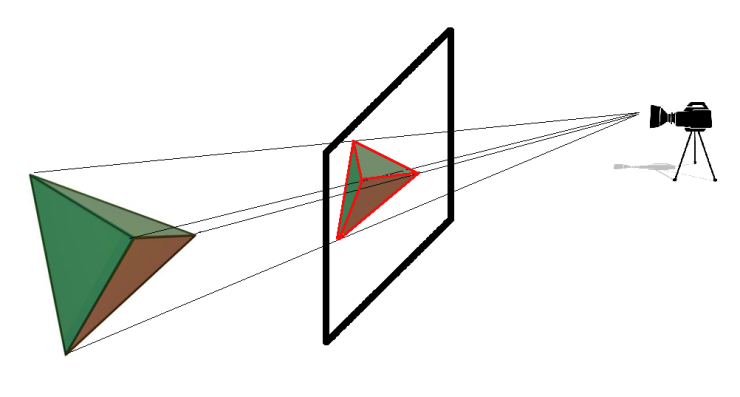
\includegraphics[scale=0.5]{Imagenes/05_Primitivas/Perspectiva01.png}
\end{center}

Disponemos de primitivas para fijar la posici\'on de la c\'amara, mientras
que la pantalla de proyecci\'on se encuentra en el punto medio entre la c\'amara
y el objeto.

\subsubsection{Entender la orientaci\'on en el mundo tridimensional}

En el plano, la tortuga la orientaci\'on se define \'unicamente por su rumbo.
Sin embargo, en el mundo tridimensional la orientaci\'on de la tortuga necesita
de tres \'angulos. Si usamos la orientaci\'on por defecto de la tortuga en 3D
(en el plano \texttt{XY} mirando hacia el semieje \texttt{Y} positivo):
\begin{description}
   \item[Balanceo:] la rotaci\'on en torno al eje \texttt{OY}
   \item[Cabeceo:] la rotaci\'on seg\'un el eje \texttt{OX}
   \item[Rumbo:] la rotaci\'on seg\'un el eje \texttt{OZ}
\end{description}
De hecho, para moverse en el mundo tridimiensional, la tortuga se comportar\'a 
de modo muy similar a un avi\'on. De nuevo, ilustremos con una imagen los 3
\'angulos:
\begin{center} \begin{tabular}{ccccc}
   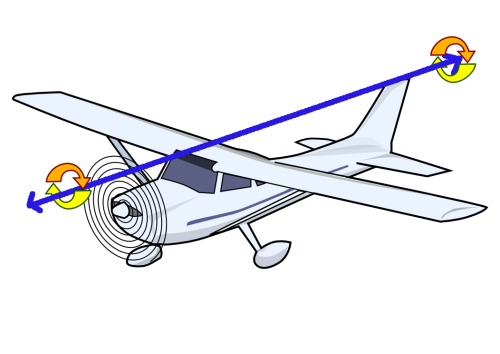
\includegraphics[scale=0.25]{Imagenes/05_Primitivas/plane-balanceo.png} & &
     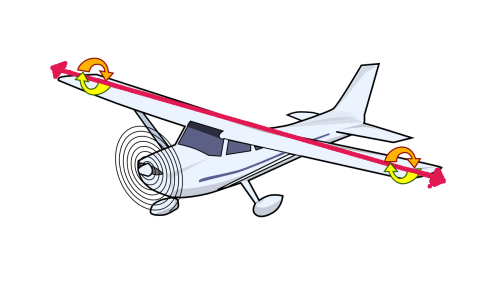
\includegraphics[scale=0.3]{Imagenes/05_Primitivas/plane-cabeceo.png} & &
       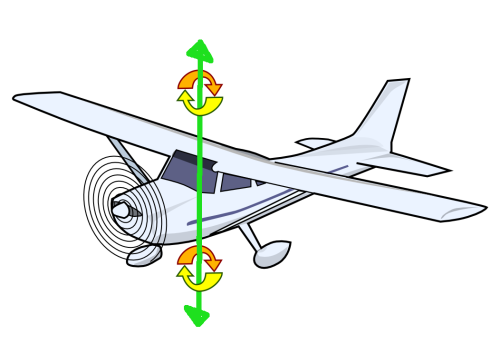
\includegraphics[scale=0.25]{Imagenes/05_Primitivas/plane-rumbo.png} \\*[0.3cm]
   \textbf{Balanceo} & & \textbf{Cabeceo} & & \textbf{Rumbo} 
\end{tabular} \end{center}

Parece bastante complicado la primera vez que se estudia, pero veremos que
muchas cosas son similares a los movimientos en el plano bidimensional. Estas
son las primitivas b\'asicas para moverse en el mundo 3D:
\begin{itemize}
   \item \texttt{avanza}, \texttt{retrocede}, \texttt{av}, \texttt{re}:
      \index{avanza@\texttt{avanza}}\index{retrocede@\texttt{retrocede}}%
      \index{av@\texttt{av}}\index{re@\texttt{re}}Id\'enticas al mundo 2D
   \item \texttt{giraderecha}, \texttt{giraizquierda}, \texttt{gd}, \texttt{gi}:
      \index{giraderecha@\texttt{giraderecha}}\index{gd@\texttt{gd}}%
      \index{giraizquierda@\texttt{giraizquierda}}\index{gi@\texttt{gi}}%
      Id\'enticas al mundo 2D, producen una rotaci\'on alrededor del eje
      transversal y vertical de la tortuga
   \item \texttt{balanceaderecha}, \texttt{bd}:
      \index{balanceaderecha@\texttt{balanceaderecha}}\index{bd@\texttt{bd}}%
      la tortuga gira \texttt{n} grados a la derecha respecto a su eje
      longitudinal 
   \item \texttt{balanceaizquierda}, \texttt{bi}:%
      \index{balanceizquierda@\texttt{balanceaizquierda}}\index{bi@\texttt{bi}}
      la tortuga gira \texttt{n} grados a la izquierda respecto a su eje
      longitudinal 
   \item \texttt{cabeceaarriba}, \texttt{subenariz}, \texttt{sn}:%
      \index{cabeceaarriba@\texttt{cabecearriba}}\index{sn@\texttt{sn}}%
      \index{subenariz@\texttt{subenariz}} La tortuga ``sube el morro''
      \texttt{n} grados respecto a su eje transversal y horizontal
   \item \texttt{cabeceaabajo}, \texttt{bajanariz}, \texttt{bn}:%
      \index{cabeceaabajo@\texttt{cabeceabajo}}\index{bn@\texttt{bn}}%
      \index{bajanariz@\texttt{bajanariz}} La tortuga ``baja el morro''
      \texttt{n} grados respecto a su eje transversal y horizontal
\end{itemize}

En el plano bidimensional, para dibujar un cuadrado de \texttt{200} pasos
de tortuga, escribimos:
\begin{verbatim}
 repite 4 [ avanza 200 giraderecha 90 ]\end{verbatim}
Estas \'ordenes siguen existiendo el mundo 3D, y el cuadrado puede
dibujarse perfectamente en modo \texttt{perspectiva}. 

\parbox{9cm}{
Si la tortuga baja ``el morro'' 90 grados, podemos dibujar otro
cuadrado, y obtenemos:\\*[0.3cm]
\texttt{borrapantalla}\\
\texttt{repite 4 [ avanza 200 giraderecha 90 ]}\\
\texttt{bajanariz 90}\\
\texttt{repite 4 [ avanza 200 giraderecha 90 ]}} \hfill 
\parbox{7cm}{\begin{center}
   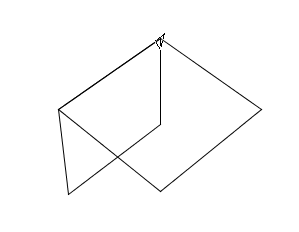
\includegraphics[scale=0.5]{Imagenes/05_Primitivas/Perspectiva02.png}
\end{center} }

Puedes (debes) probar otros ejemplos para entender perfectamente la
orientaci\'on de la tortuga y el uso de los \'angulos y !`convertirte en
un experto! \\

\noindent Tambi\'en debes entender que las tres primitivas que controlan la
rotaci\'on en 3D est\'an relacionadas entre s\'i; por ejemplo, al ejecutar:
\begin{verbatim}
 borrapantalla
 balanceaizquierda 90 subenariz 90 balanceaderecha 90\end{verbatim}
El movimiento de la tortuga es equivalente a:
\begin{verbatim}
 giraizquierda 90\end{verbatim}
(Puedes probar con tu mano si no lo entiendes bien)

\subsubsection{Primitivas disponibles tanto en 2D como 3D}

Las siguientes primitivas est\'an disponibles tanto en el plano como en
el mundo 3D. La \'unica diferencia son los argumentos admitidos por las
primitivas. \\

\noindent Estas precisan de los mismos argumentos que en el plano:
\begin{center}\begin{tabular}{ccccc}
   \texttt{c\'irculo}\index{c\'irculo@\texttt{c\'irculo}}    & &
   \texttt{arco}\index{arco@\texttt{arco}}             & &
   \texttt{centro}\index{centro@\texttt{centro}}       \\
   \texttt{ponx}\index{ponx@\texttt{ponx}}             & &
   \texttt{pony}\index{pony@\texttt{pony}}             & &
   \texttt{rumbo}\index{rumbo@\texttt{rumbo}}          \\
   \texttt{ponrumbo}\index{ponrumbo@\texttt{ponrumbo}} & &
   \texttt{rotula}\index{rotula@\texttt{rotula}}       & &
   \texttt{largoetiqueta}\index{largoetiqueta@\texttt{largoetiqueta}}
\end{tabular}\end{center}

\noindent Las siguientes primitivas siguen esperando una lista como
argumento, pero ahora debe contener \textbf{tres} argumentos,
correspondientes a las tres coordenadas de un punto en el espacio:
\texttt{[x y z]}.
\begin{center}\begin{tabular}{ccccc}
   \texttt{hacia}\index{hacia@\texttt{hacia}}              & &
   \texttt{distancia}\index{distancia@\texttt{distancia}}  & &
   \texttt{pos}, \texttt{posici\'on}
      \index{posici\'on@\texttt{posici\'on}}\index{pos@\texttt{pos}} \\
   \texttt{ponpos}, \texttt{ponposici\'on}
      \index{ponposici\'on@\texttt{ponposici\'on}}\index{ponpos@\texttt{ponpos}} & &
   \texttt{punto} \index{punto@\texttt{punto}}              & &
\end{tabular}\end{center}

\subsubsection{Primitivas s\'olo disponibles en 3D}

\begin{itemize}
   \item \texttt{ponxyz}\index{ponxyz@\texttt{ponxyz}}
      Esta primitiva mueve a la tortuga al punto elegido. Esta primitiva
      espera tres argumentos que representan las coordenadas del punto.

      \texttt{ponxyz} es muy similar a \texttt{ponposici\'on}, pero las
      coordenadas no est\'an escritos en una lista.

      Ejemplo, \texttt{ponxyz -100 200 50} traslada a la tortuga hasta el
      punto \texttt{x = -100}; \texttt{y = 200}; \texttt{z = 50}
   \item \texttt{ponz}\index{ponz@\texttt{ponz}}
      Esta primitiva mueve a la tortuga al punto de ``altura'' o
      ``profundidad'' (desconozco si el t\'ermino \textit{applikate} usado
      en Alemania tiene traducci\'on al castellano m\'as all\'a de
      \textbf{tercera coordenada}) dada.
      \texttt{ponz} recibe un n\'umero como argumento, de modo id\'entico a
      \texttt{ponx} y \texttt{pony}
   \item \texttt{ponorientaci\'on}\index{ponorientaci\'on@\texttt{ponorientaci\'on}}
      Fija la orientaci\'on de la tortuga. Esta primitiva espera una lista que
      contiene tres n\'umeros: \texttt{[balanceo cabeceo rumbo]}

      Ejemplo: \texttt{ponorientaci\'on [100 0 58]}: la tortuga tendr\'a 
      balanceo: 100 grados, cabeceo: 0 grados y rumbo: 58 grados.

      Por supuesto, el orden de los n\'umeros es importante. Si, por ejemplo,
      el valor de la orientaci\'on es \texttt{[100 20 90]}, esto significa que
      si quieres esa misma orientaci\'on partiendo del origen (despu\'es de un
      \texttt{borrapantalla}, por ejemplo) deber\'as escribir la siguiente
      secuencia:
      \begin{verbatim}
  cabeceaderecha 100
  subenariz 20
  giraderecha 90\end{verbatim}
      Si en esta instrucci\'on cambiamos el orden, no obtendremos la orientaci\'on
      deseada.
   \item \texttt{orientaci\'on}\index{orientaci\'on@\texttt{orientaci\'on}}
      Devuelve la orientaci\'on de la tortuga en una lista que contiene:
      \texttt{[balanceo cabeceo rumbo]} 
   \item \texttt{ponbalanceo}\index{ponbalanceo@\texttt{ponbalanceo}}
      La tortuga gira en torno a su eje longitudinal y adquiere el \'angulo
      de balanceo elegido.
   \item \texttt{balanceo}\index{balanceo@\texttt{balanceo}}
      Devuelve el valor actual del balanceo
   \item \texttt{ponbalanceo}\index{poncabeceo@\texttt{poncabeceo}} La tortuga
      gira en torno a su eje transversal, y se orienta con el \'angulo de cabeceo
      indicado.
   \item \texttt{balanceo}\index{cabeceo@\texttt{cabeceo}}
      Devuelve el valor actual del cabeceo
\end{itemize}

\subsubsection{Visor 3D} 

\textsc{XLogo} incluye un visor 3D que permite visualizar los dibujos realizados
en tres dimensiones. Este m\'odulo usa las librer\'ias de \textsc{Java3D}, por lo
tanto es necesario tener instalado todo el \textsc{Java3D}. \\

\noindent Las reglas a tener en cuenta para utilizar el Visor 3D son:

Al crear una figura geom\'etrica sobre el \'Area de Dibujo, hay que indicar al
Visor 3D qu\'e formas desea grabar para una futura visualizaci\'on. Es posible
grabar pol\'igonos (superficies), l\'ineas, puntos o texto. Para utilizar esta
funci\'on, las primitivas son:
\begin{itemize}
   \item \texttt{empiezapol\'igono}, \texttt{definepol\'igono}, \texttt{defpoli}:%
      \index{empiezapol\'igono@\texttt{empiezapol\'igono}}%
      \index{definepol\'igono@\texttt{definepol\'igono}}%
      \index{defpoli@\texttt{defpoli}}
      Los movimientos de la tortuga posteriores a esta llamada se guardan para
      crear un pol\'igono.
   \item \texttt{finpol\'igono}, \texttt{finpoli}:%
      \index{finpol\'igono@\texttt{finpol\'igono}}\index{finpoli@\texttt{finpoli}}
      Desde la ejecuci\'on de \texttt{definepol\'igono}, la tortuga habr\'a
      pasado por varios v\'ertices. Este pol\'igono se habr\'a ``registrado'' y
      su color se definir\'a en funci\'on del color de todos sus v\'ertices.

      Esta primitiva finaliza el pol\'igono.
   \item \texttt{empiezal\'inea}, \texttt{definel\'inea}, \texttt{defl\'inea}:%
      \index{empiezal\'inea@\texttt{empiezal\'inea}}%
      \index{definel\'inea@\texttt{definel\'inea}}%
      \index{defl\'inea@\texttt{defl\'inea}}
      Los movimientos de la tortuga posteriores a esta llamada se guardan para
      crear un quebrado, es decir, una l\'inea con varios v\'ertices que no tiene
      por qu\'e ser cerrada.
   \item \texttt{finl\'inea}:\index{finl\'inea@\texttt{finl\'inea}}
      Desde la ejecuci\'on de \texttt{definel\'inea}, la tortuga habr\'a
      pasado por varios v\'ertices. Se guardar\'a esta l\'inea y su color se
      definir\'a en funci\'on del color de todos sus v\'ertices.

      Esta primitiva finaliza la definici\'on del quebrado
   \item \texttt{empiezapunto}, \texttt{definepunto}, \texttt{defpto}:%
      \index{empiezapunto@\texttt{empiezapunto}}%
      \index{definepunto@\texttt{definepunto}}%
      \index{defpto@\texttt{defpto}}
      Los movimientos posteriores de la tortuga definen los v\'erices de un
      quebrado cuyos v\'ertices se guardan para crear un conjunto de puntos.
   \item \texttt{finpunto}, \texttt{finpto}:%
      \index{finpunto@\texttt{finpunto}}%
      \index{finpto@\texttt{finpto}} Esta primitiva 
      finaliza la definici\'on del conjunto de puntos.
   \item \texttt{empiezatexto}, \texttt{definetexto}, \texttt{deftxt}:%
      \index{empiezatexto@\texttt{empiezatexto}}%
      \index{definetexto@\texttt{definetexto}}%
      \index{deftxt@\texttt{deftxt}}
      Cada vez que el usuario muestre un texto sobre el \'Area de Dibujo con
      la primitiva \texttt{rotula}, se almacenar\'a y luego ser\'a representada
      por el visor 3D.
   \item \texttt{fintexto}, \texttt{fintxt}:%
      \index{fintexto@\texttt{fintexto}}%
      \index{fintxt@\texttt{fintxt}} Esta primitiva
      la grabaci\'on de texto.
   \item \texttt{vista3d}, \texttt{vistapol\'igono}%
      \index{vista3d@\texttt{vista3d}}%
      \index{vistapol\'igono@\texttt{vistapol\'igono}}
      Inicia el visor 3D, todos los objetos guardados se dibujan en una nueva
      ventana.

      Disponemos de controles para mover la ``c\'amara'' que muestra la escena:
      \begin{itemize}
         \item Para hacer rotar la imagen haciendo \textit{click} con el bot\'on
            izquierdo del rat\'on y arrastrando.
         \item Para desplazar la imagen haciendo \textit{click} con el bot\'on
            derecho del rat\'on y arrastrando.
         \item Para hacer \textit{zoom} sobre la escena, usaremos la rueda del
            rat\'on
      \end{itemize}
\end{itemize}

\subsubsection{Dibujando un cubo}

Todas las caras miden 400 pasos de tortuga. El programa es: \\

\noindent\texttt{para cuadrado} \\
\texttt{\# Grabamos los v\'ertices del cuadrado} \\
\verb+  +\texttt{empiezapol\'igono} \\
\verb+  +\texttt{repite 4 [ avanza 400 giraderecha 90 ]} \\
\verb+  +\texttt{finpol\'igono} \\
\texttt{fin} \\

\noindent\texttt{para cubosimple} \\
\texttt{\# Cubo Amarillo} \\
\verb+  +\texttt{borrapantalla perspectiva} \\
\verb+  +\texttt{poncolorl\'apiz amarillo} \\
\texttt{\# Caras laterales} \\
\verb+  +\texttt{repite 4} \\
\verb+    +\texttt{[ cuadrado subel\'apiz} \\
\verb+      +\texttt{giraderecha 90 avanza 400 giraizquierda 90} \\
\verb+      +\texttt{balanceaderecha 90 bajal\'apiz ]} \\
\texttt{\# Parte inferior} \\
\verb+  +\texttt{bajanariz 90 cuadrado subenariz 90} \\
\texttt{\# Cara Superior} \\
\verb+  +\texttt{avanza 400 bajanariz 90 cuadrado} \\
\texttt{\# Visualizaci\'on} \\
\verb+  +\texttt{vista3d} \\
\texttt{fin} \\

Estamos listos a ejecutar el comando: \verb+cubosimple+:
\begin{center}
   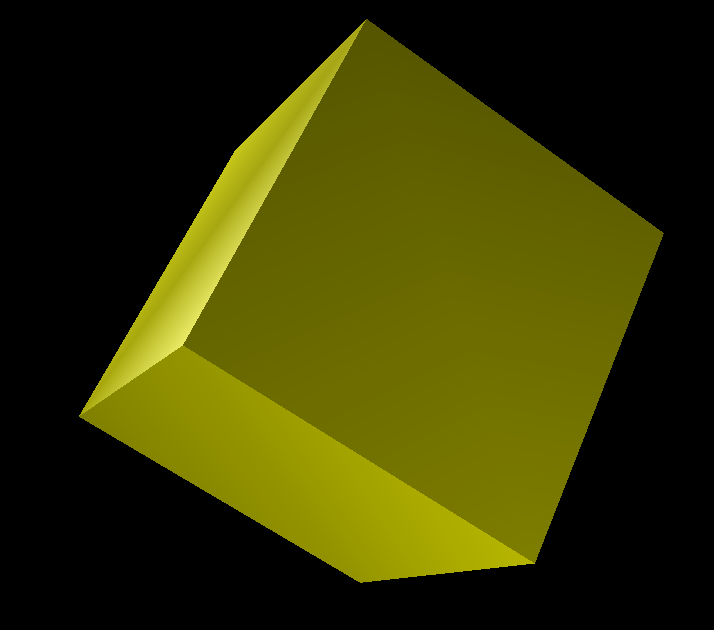
\includegraphics[scale=0.2]{Imagenes/05_Primitivas/3dCube1.png}
\end{center}

Al sustituir en el procedimiento \verb+cuadrado+, \texttt{empiezapol\'igono}
por \texttt{empiezal\'inea}, y \texttt{finpoligono} por \texttt{finl\'inea}:
\begin{center}
   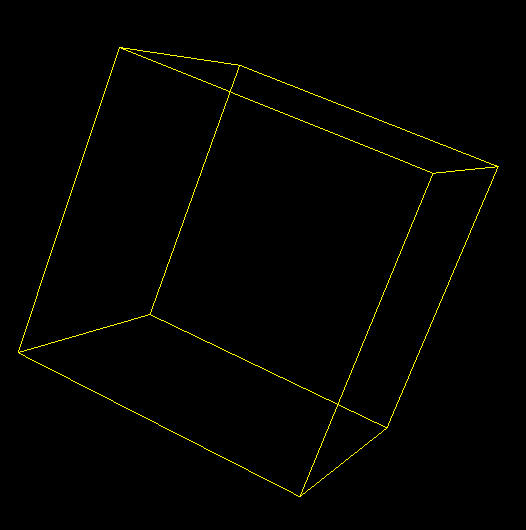
\includegraphics[scale=0.2]{Imagenes/05_Primitivas/3dCube2.png}
\end{center}

Si hubi\'eramos usado \texttt{empiezapunto} y \texttt{finpunto} en lugar de
\texttt{empiezal\'inea} y \texttt{finl\'inea}, deber\'iamos ver en la pantalla
s\'olo los ocho v\'ertices del cubo. \\

\noindent Estas primitivas son muy \'utiles para mostrar el conjunto de puntos
en el espacio 3D. \\
% No merece la pena imagen

\noindent En todos los casos, en el \'Area de Dibujo se muestran las aristas
del cubo que luego se ver\'a ``macizo'' con el Visor:
\begin{center}
   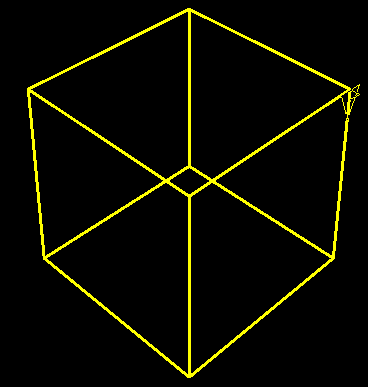
\includegraphics[scale=0.3]{Imagenes/05_Primitivas/CuboSimple03.png}
\end{center}

\subsubsection{Efectos de luz y niebla}
\index{Efectos de luz y niebla}

Desde la versi\'on 0.9.93 se pueden a\~nadir efectos art\'isticos a las
im\'agenes generadas en el Visor. Estos pueden ser efectos de luz y de niebla,
y se accede a ellos con los botones presentes en el visor 3D.
\begin{center}
   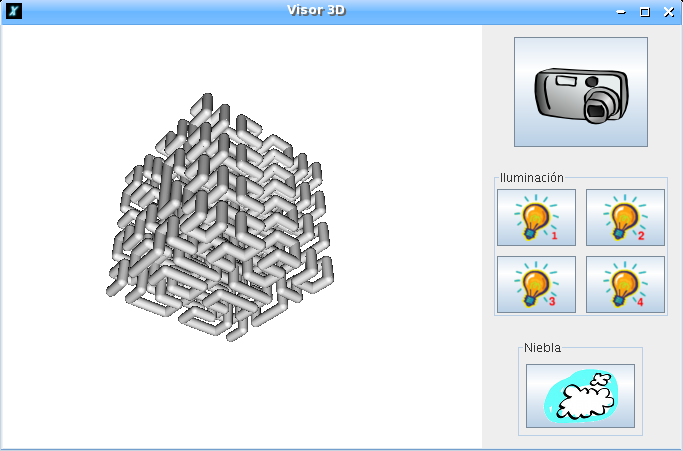
\includegraphics[scale=0.25]{Imagenes/05_Primitivas/Visor3D.png}
\end{center}

\subsubsection*{Efectos de luz}

Se pueden utilizar cuatro tipos de luz en las im\'agenes en tres dimensiones,
a las que se accede haciendo \textit{click} en uno de los cuatro botones mostrados
bajo la leyenda \texttt{Iluminaci\'on}. \\ 

Al trazar por primera vez una imagen en 3D s\'olo se utilizan dos tipos de luz,
ambos \textbf{Luz Puntual}, pero pulsando en cualquiera de los cuatro botones de
\texttt{Iluminaci\'on}, aparece el siguiente cuadro de di\'alogo:
\begin{center}
   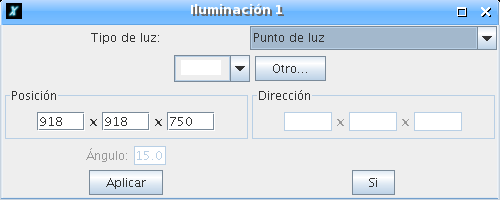
\includegraphics[scale=0.4]{Imagenes/05_Primitivas/Iluminacion1.png}
\end{center}
donde podemos elegir entre los siguientes tipos de luz:
\begin{description}
   \item[Luz Ambiente:] Luz uniforme de la que s\'olo puede modificarse el color
      \index{Luz Ambiental}
   \item[Luz Direccional:] Se genera respecto a una direcci\'on fija. Se parece a la
      luz ambiente cuando la fuente est\'a muy lejos del objeto (por ejemplo, el sol)
      \index{Luz Direccional} 
   \item[Punto de Luz:] La fuente est\'a en una posici\'on determinada, como en el
      caso de un faro.\index{Punto de Luz}
   \item[Foco:] Es como el punto de luz, pero el haz de luz se abre formando un cono
      cuya abertura debe fijarse.\index{Foco}
\end{description}
La mejor forma de entenderlo, es practicar con ello.
\begin{center}
   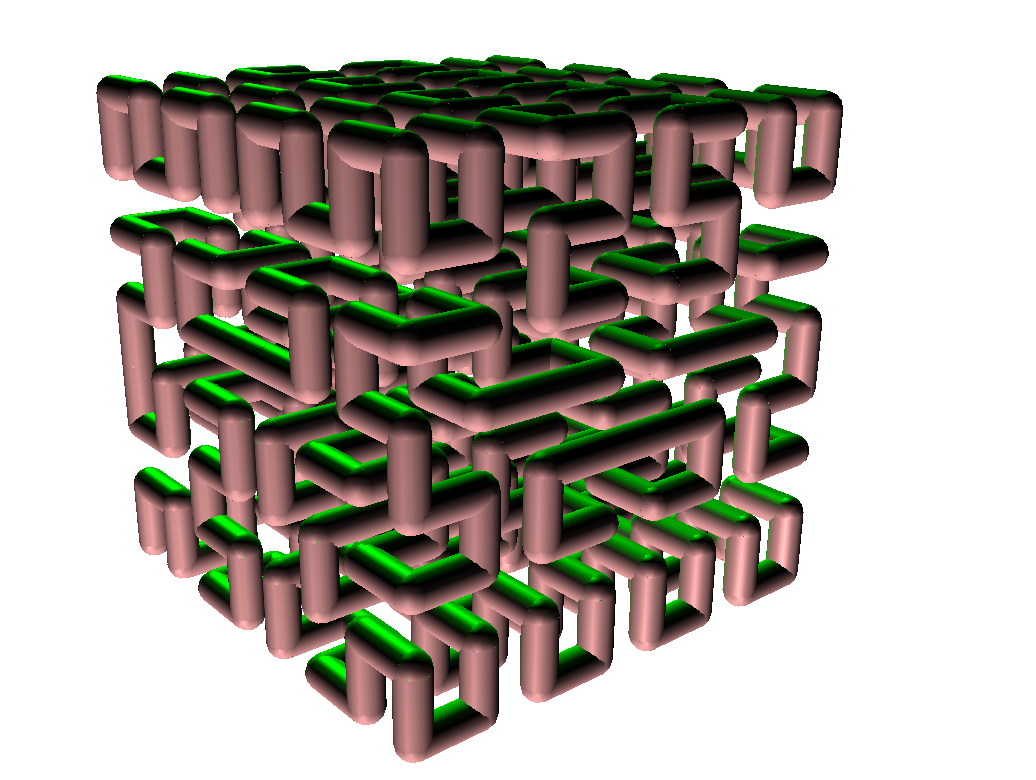
\includegraphics[scale=0.2]{Imagenes/05_Primitivas/hilbert.png}
\end{center}

\subsubsection*{Efectos de niebla}

Se pueden a\~nadir efectos de niebla en la imagen tridimensional. Pulsa el bot\'on
con ``nubes'' y obtendr\'as este cuadro de di\'alogo:
\begin{center}
   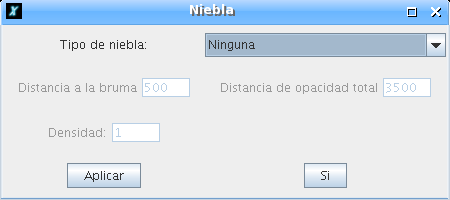
\includegraphics[scale=0.3]{Imagenes/05_Primitivas/Niebla.png}
\end{center}
Disponemos de dos tipos de niebla:
\begin{description}
   \item[Niebla Lineal o progresiva:] La imagen se va difuminando de modo lineal,
      pudiendo variar dos par\'ametros:\index{Niebla lineal}
      \begin{itemize}
         \item La distancia a la que empieza la niebla 
         \item La distancia a la que la niebla no deja ver nada (opacidad total)
      \end{itemize}
   \item[Niebla Densa:] La niebla es uniforme en toda la escena, y s\'olo necesitamos
      especificar la densidad de la misma.\index{Niebla densa}
\end{description}
Este es un ejemplo con niebla lineal:
\begin{center}
   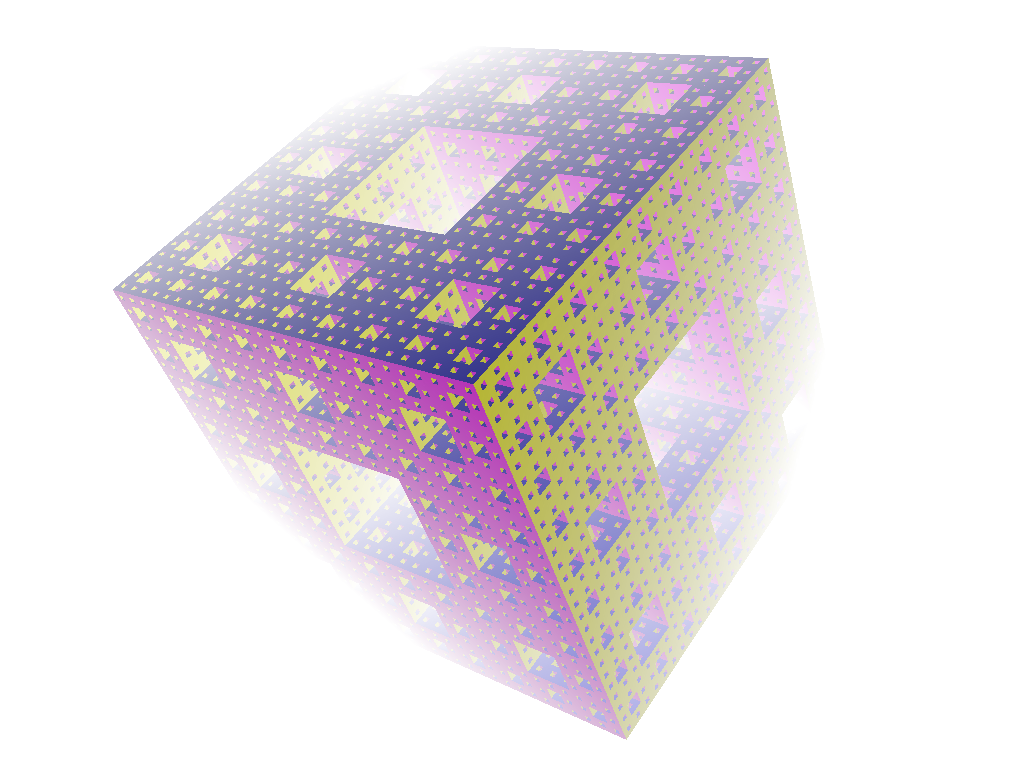
\includegraphics[scale=0.2]{Imagenes/05_Primitivas/EjemploNiebla.png}
\end{center}

\subsection{Acerca de los colores}
   \label{AcercaColores}
   \index{Colores}

El color en \textsc{XLogo} est\'a especificado por una lista de tres n\'umeros
\texttt{[r v a]} comprendidos entre 0 y 255. El n\'umero \texttt{r} es
el componente rojo, \texttt{v} el verde y \texttt{a} el azul
(\texttt{[r g b]} en ingl\'es). \textsc{XLogo} tiene 17 colores predefinidos, a
los que se puede referir con un n\'umero, con su lista \texttt{[r~v~a]}
o con una primitiva. Las primitivas correspondientes son:
\begin{center} \begin{longtable}{|*{4}{c|}} \hline  
    \textbf{N\'umero} & \textbf{Primitiva} & \textbf{[R V A]} & \textbf{Color}
             \\ \endhead \hline
    0 & \texttt{negro} \index{negro@\texttt{negro}}
      & \texttt{[0   0   0]} & \begin{minipage}[m]{1.5cm} \begin{center}
           \vspace{0.2cm} %\textcolor{black}{\rule{1.0cm}{0.5cm}} 
              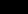
\includegraphics{Imagenes/05_Primitivas/00_negro.png}
           \vspace{0.2cm} \end{center} \end{minipage} \\ \hline
    1 & \texttt{rojo} \index{rojo@\texttt{rojo}}
      & \texttt{[255  0   0]} & \begin{minipage}[m]{1.5cm} \begin{center}
                 \vspace{0.2cm} %\textcolor{red}{\rule{1.0cm}{0.5cm}} 
              
\includegraphics{Imagenes/05_Primitivas/01_rojo.png}
                 \vspace{0.2cm} \end{center} \end{minipage} \\ \hline
    2 & \texttt{verde} \index{verde@\texttt{verde}}
      & \texttt{[0  255  0]} & \begin{minipage}[m]{1.5cm} \begin{center}
                \vspace{0.2cm} %\textcolor{green}{\rule{1.0cm}{0.5cm}} 
              
\includegraphics{Imagenes/05_Primitivas/02_verde.png}
                \vspace{0.2cm} \end{center} \end{minipage} \\ \hline
    3 & \texttt{amarillo} \index{amarillo@\texttt{amarillo}}
      & \texttt{[255 255  0]} &  \begin{minipage}[m]{1.5cm} \begin{center}
               \vspace{0.2cm} %\textcolor{yellow}{\rule{1.0cm}{0.5cm}} 
              
\includegraphics{Imagenes/05_Primitivas/03_amarillo.png}
               \vspace{0.2cm} \end{center} \end{minipage} \\ \hline
    4 & \texttt{azul} \index{azul@\texttt{azul}}
      & \texttt{[0   0  255]} & \begin{minipage}[m]{1.5cm} \begin{center}
                 \vspace{0.2cm} %\textcolor{blue}{\rule{1.0cm}{0.5cm}}
              
\includegraphics{Imagenes/05_Primitivas/04_azul.png}
                 \vspace{0.2cm} \end{center} \end{minipage} \\ \hline
    5 & \texttt{magenta} \index{magenta@\texttt{magenta}}
      & \texttt{[255  0  255]} & \begin{minipage}[m]{1.5cm} \begin{center}
              \vspace{0.2cm} %\textcolor{magenta}{\rule{1.0cm}{0.5cm}} 
              
\includegraphics{Imagenes/05_Primitivas/05_magenta.png}
              \vspace{0.2cm} \end{center} \end{minipage} \\ \hline
    6 & \texttt{cyan} \index{cyan@\texttt{cyan}}
      & \texttt{[0  255 255]} & \begin{minipage}[m]{1.5cm} \begin{center}
                 \vspace{0.2cm} %\textcolor{cyan}{\rule{1.0cm}{0.5cm}}
              
\includegraphics{Imagenes/05_Primitivas/06_cyan.png}
                 \vspace{0.2cm} \end{center} \end{minipage} \\ \hline
    7 & \texttt{blanco} \index{blanco@\texttt{blanco}}
      & \texttt{[255 255 255]} & \begin{minipage}[m]{1.5cm} \begin{center}
                \vspace{0.2cm} %\textcolor{white}{\rule{1.0cm}{0.5cm}}
              
\includegraphics{Imagenes/05_Primitivas/07_blanco.png}
                \vspace{0.2cm} \end{center} \end{minipage} \\ \hline
    8 & \texttt{gris} \index{gris@\texttt{gris}}
      & \texttt{[128 128 128]} &  \begin{minipage}[m]{1.5cm} \begin{center}
                 \vspace{0.2cm} %\definecolor{grey}{rgb}{0.5,0.5,0.5}
%                    \textcolor{grey}{\rule{1.0cm}{0.5cm}} 
              
\includegraphics{Imagenes/05_Primitivas/08_gris.png}
                 \vspace{0.2cm} \end{center}
                              \end{minipage} \\ \hline
    9 & \texttt{grisclaro} \index{grisclaro@\texttt{grisclaro}}
      & \texttt{[192 192 192]} & \begin{minipage}[m]{1.5cm} \begin{center}
                 \vspace{0.2cm} %\definecolor{lightgrey}{rgb}{0.75,0.75,0.75}
%                      \textcolor{lightgrey}{\rule{1.0cm}{0.5cm}}
              
\includegraphics{Imagenes/05_Primitivas/09_grisclaro.png}
                   \vspace{0.2cm} \end{center}
                              \end{minipage} \\ \hline
   10 & \texttt{rojooscuro} \index{rojooscuro@\texttt{rojooscuro}}
      & \texttt{[128  0   0]} &  \begin{minipage}[m]{1.5cm} \begin{center}
                 \vspace{0.2cm} % \definecolor{darkred}{rgb}{0.5,0,0}
%                    \textcolor{darkred}{\rule{1.0cm}{0.5cm}}
              
\includegraphics{Imagenes/05_Primitivas/10_rojooscuro.png}
                   \vspace{0.2cm} \end{center}
                              \end{minipage} \\ \hline
   11 & \texttt{verdeoscuro} \index{verdeoscuro@\texttt{verdeoscuro}}
      & \texttt{[0  128  0]} &  \begin{minipage}[m]{1.5cm} \begin{center}
                 \vspace{0.2cm} %\definecolor{darkgreen}{rgb}{0,0.5,0}
%                     \textcolor{darkgreen}{\rule{1.0cm}{0.5cm}} 
              
\includegraphics{Imagenes/05_Primitivas/11_verdeoscuro.png}
                   \vspace{0.2cm} \end{center}
                              \end{minipage} \\ \hline
   12 & \texttt{azuloscuro} \index{azuloscuro@\texttt{azuloscuro}}
      & \texttt{[0   0  128]} &  \begin{minipage}[m]{1.5cm} \begin{center}
                 \vspace{0.2cm} %\definecolor{darkblue}{rgb}{0,0,0.5}
%                           \textcolor{darkblue}{\rule{1.0cm}{0.5cm}} 
              
\includegraphics{Imagenes/05_Primitivas/12_azuloscuro.png}
                      \vspace{0.2cm} \end{center}
                              \end{minipage} \\ \hline
   13 & \texttt{naranja} \index{naranja@\texttt{naranja}}
      & \texttt{[255 200  0]} &  \begin{minipage}[m]{1.5cm} \begin{center}
                 \vspace{0.2cm} %\definecolor{orange}{rgb}{1,0.78,0}
%                   \textcolor{orange}{\rule{1.0cm}{0.5cm}}
              
\includegraphics{Imagenes/05_Primitivas/13_naranja.png}
                   \vspace{0.2cm} \end{center}
                              \end{minipage} \\ \hline
   14 & \texttt{rosa} \index{rosa@\texttt{rosa}}
      & \texttt{[255 175 175]} & \begin{minipage}[m]{1.5cm} \begin{center}
                 \vspace{0.2cm} % \definecolor{pink}{rgb}{1,0.70,0.70}
%                           \textcolor{pink}{\rule{1.0cm}{0.5cm}}
              
\includegraphics{Imagenes/05_Primitivas/14_rosa.png}
                     \vspace{0.2cm} \end{center}
                              \end{minipage} \\ \hline
   15 & \texttt{violeta} \index{violeta@\texttt{violeta}}
      & \texttt{[128  0  255]} & \begin{minipage}[m]{1.5cm} \begin{center}
                 \vspace{0.2cm} % \definecolor{purple}{rgb}{0.5,0,1}
%                        \textcolor{purple}{\rule{1.0cm}{0.5cm}}
              
\includegraphics{Imagenes/05_Primitivas/15_violeta.png}
                    \vspace{0.2cm} \end{center}
                              \end{minipage} \\ \hline
   16 & \texttt{marr\'on} \index{marr\'on@\texttt{marr\'on}}
      & \texttt{[153 102  0]} &  \begin{minipage}[m]{1.5cm} \begin{center}
                 \vspace{0.2cm} \definecolor{brown}{rgb}{0.6,0.4,0}
%                       \textcolor{brown}{\rule{1.0cm}{0.5cm}}
              
\includegraphics{Imagenes/05_Primitivas/16_marron.png}
                    \vspace{0.2cm} \end{center}
                       \end{minipage} \\ \hline
\end{longtable}\end{center}

\noindent \textbf{Ejemplo:} Estas tres \'ordenes son la misma:

   \texttt{poncolorl\'apiz naranja}

   \texttt{poncolorl\'apiz 13}

   \texttt{poncolorl\'apiz [255 200 0]}

\noindent Veremos un ejemplo de su uso en la secci\'on \ref{EjColores}

\subsection{Animaci\'on}
   \label{animaci\'on}
   \index{Animaci\'on}

Existen dos primitivas llamadas \texttt{animaci\'on}%
\index{animaci\'on@\texttt{animaci\'on}}%
\index{detieneanimaci\'on@\texttt{detieneanimaci\'on}}
y \texttt{refresca} (por compatibilidad con otras versiones de
\textsc{Logo} se mantiene la forma en infinitivo \texttt{refrescar})%
\index{refrescar@\texttt{refrescar}}% 
\index{refresca@\texttt{refresca}} que permiten
escribir \'ordenes sin que la tortuga las realice.

\begin{center} \begin{longtable}{|m{4cm}|m{9cm}|} \hline 
   \multicolumn{1}{|c|}{\textbf{Primitivas}} &
         \multicolumn{1}{c|}{\textbf{Uso}} \\ \endhead \hline 
   \texttt{animaci\'on} &  
      Se accede al modo de animaci\'on. \\ \hline 
   \texttt{detieneanimaci\'on} & 
      Detiene el modo animaci\'on, retornando al modo \textit{normal}.\\ \hline 
   \texttt{refresca} &  
      En modo de animaci\'on, ejecuta las \'ordenes y actualiza la imagen 
           \\ \hline
\end{longtable} \end{center}

Mientras se escriben las \'ordenes en el modo de animaci\'on (una c\'amara
de cine aparece a la izquierda del \textbf{Hist\'orico de Comandos}),
\'estas no son ejecutadas en el \textbf{\'Area de Dibujo} sino que son
almacenadas en memoria hasta que se introduce la orden \texttt{refresca}.

\begin{center}
   
\includegraphics[scale=2.5]{Imagenes/05_Primitivas/animation.png}
\end{center}
Haciendo \textit{click} en este icono, se detiene el modo de animaci\'on,
sin necesidad de usar la primitiva \texttt{detieneanimaci\'on}.

Esto es muy \'util para crear animaci\'ones o conseguir que los dibujos
se realicen r\'apidamente.

\subsection{Propiedades del Hist\'orico de Comandos}
   \label{Propiedades-Historico}

Esta tercera tabla define las primitivas que permiten ajustar las
propiedades de texto del \'area del hist\'orico de comandos. Aquellas
primitivas que controlan el color y tama\~no de este \'area, s\'olo est\'an
disponibles para ser usadas por las primitivas \texttt{escribe} y
\texttt{tipea}.

\begin{center}\begin{longtable}{|m{35mm}|m{25mm}|m{9cm}|} \hline 
\multicolumn{1}{|c|}{\textbf{Primitivas}} &
   \multicolumn{1}{c|}{\textbf{Argumentos}} &
      \multicolumn{1}{c|}{\textbf{Uso}} \\ \endhead \hline
   \texttt{borratexto}, \index{borratexto@\texttt{borratexto}}
     \texttt{bt} \index{bt@\texttt{bt}} & \texttt{no} &
        Borra el \textbf{\'Area de comandos}, y el \'area del
        \textbf{Hist\'orico de comandos}. \\ \hline 
   \texttt{escribe}, \index{escribe@\texttt{escribe}}
     \texttt{es} \index{es@\texttt{es}} & 
        \texttt{a: n\'umero, palabra o lista} &
        Muestra en el \textbf{Hist\'orico de Comandos} el argumento indicado,
        \texttt{a}.\\ \hline 
   \texttt{tipea}\index{tipea@\texttt{tipea}},
      \texttt{mecanograf\'ia} \index{mecanograf\'ia@\texttt{mecanograf\'ia}}  & 
      \texttt{a: n\'umero, palabra o lista} &
        Id\'entico a \texttt{escribe}, pero el cursor queda en la l\'inea donde
        se mostr\'o el contenido del argmento. \\ \hline 
   \texttt{ponfuentetexto}, \index{ponfuentetexto@\texttt{ponfuentetexto}}
      \texttt{pft} \index{pft@\texttt{pft}} & \texttt{n: n\'umero} &
        Define el tama\~no de la tipograf\'ia del \'area del
        \textbf{Hist\'orico de comandos}. S\'olo disponible para ser usada
        por la primitiva \texttt{escribe}. \\ \hline 
   \texttt{fuentetexto}, \index{fuentetexto@\texttt{fuentetexto}}
     \texttt{ftexto} \index{ftexto@\texttt{ftexto}} & \texttt{no} &
        Devuelve el tama\~no de la tipograf\'ia usada por la primitiva
        \texttt{escribe}. \\ \hline 
   \texttt{poncolortexto}, \index{poncolortexto@\texttt{poncolortexto}}
     \texttt{pctexto} \index{pctexto@\texttt{pctexto}} & 
        \texttt{a: n\'umero o lista} &
        Define el color de la tipograf\'ia del \'area del
        \textbf{Hist\'orico de comandos}. S\'olo disponible para ser
        usada por la primitiva \texttt{escribe}.\\ \hline 
   \texttt{colortexto} \index{colortexto@\texttt{colortexto}} & \texttt{no} &
        Devuelve el color de la tipograf\'ia usada por la primitiva
        \texttt{escribe} en el \'area del \textbf{Hist\'orico de comandos}.\\ \hline
   \texttt{ponnombrefuentetexto}, 
      \index{ponnombrefuentetexto@\texttt{ponnombrefuentetexto}}
     \texttt{pnft} \index{pnft@\texttt{pnft}} & \texttt{n: n\'umero} &
        Selecciona la tipograf\'ia n\'umero \texttt{n} para escribir en
        el \'area del \textbf{Hist\'orico de comandos} con la primitiva
        \texttt{escribe}. Puedes encontrar la relaci\'on entre fuente y
        n\'umero en el men\'u \textbf{Herramientas $\rightarrow$ Preferencias
        $\rightarrow$ Fuente.} \\ \hline 
   \texttt{nombrefuentetexto},
       \index{nombrefuentetexto@\texttt{nombrefuentetexto}}
     \texttt{nft} \index{nft@\texttt{nft}} & \texttt{no} &
        Devuelve una lista con dos elementos. El primero es un n\'umero
        correspondiente a la fuente utilizada para escribir en el \'area
        del \textbf{Hist\'orico de comandos} con la primitiva \texttt{escribe}.
        El segundo elemento es una lista que contiene el nombre de la fuente.
                        \\ \hline
   \texttt{ponestilo}, \index{ponestilo@\texttt{ponestilo}}
     \texttt{pest} \index{pest@\texttt{pest}} & \texttt{lista o palabra} &
        Define los efectos de fuente para los comandos en el
        \textbf{Hist\'orico de comandos}. Puedes elegir entre siete
        estilos: \texttt{ninguno}, \index{ninguno@\texttt{ninguno}}
        \texttt{negrita}, \index{negrita@\texttt{negrita}}
%        \texttt{it\'alica}\index{it\'alica@\texttt{it\'alica}} o
        \texttt{cursiva}\index{cursiva@\texttt{cursiva}},
        \texttt{tachado}, \index{tachado@\texttt{tachado}}
        \texttt{subrayado}, \index{subrayado@\texttt{subrayado}}
        \texttt{super\'indice} \index{super\'indice@\texttt{super\'indice}} y
        \texttt{sub\'indice}. \index{sub\'indice@\texttt{sub\'indice}}
        Si quieres aplicar varios estilos a la vez, escr\'ibelos en una
        lista. Mira los ejemplos al final de la tabla.
                        \\ \hline
   \texttt{estilo}, \index{estilo@\texttt{estilo}}
%     \texttt{est} \index{est@\texttt{est}} 
      & \texttt{no} &
        Devuelve una lista que contiene todos los efectos de fuente
        utilizados por las primitivas \texttt{escribe} y \texttt{tipea}.
                        \\ \hline
   \texttt{ponseparaci\'on}, \index{ponseparaci\'on@\texttt{ponseparaci\'on}}
     \texttt{ponsep}%
     \index{ponsep@\texttt{ponsep}} & 
       \texttt{n: n\'umero comprendido entre 0 y 1} &
        Determina la proporci\'on de pantalla ocupada por el
        \textbf{\'Area de Dibujo} y el \textbf{Hist\'orico de Comandos}.
        Si \texttt{n} vale 1, el \textbf{\'Area de Dibujo} ocupar\'a toda
        la pantalla. Si \texttt{n} vale 0, ser\'a el \textbf{Hist\'orico}
        quien la ocupe.\\ \hline 
   \texttt{separaci\'on} \index{separaci\'on@\texttt{separaci\'on}} &
      \texttt{no} &
        Devuelve el valor de la proporci\'on de pantalla ocupada por el
        \textbf{\'Area de Dibujo} y el \textbf{Hist\'orico de Comandos}.
                        \\ \hline
\end{longtable} \end{center}
\begin{quote}
   \noindent \textbf{Ejemplos de estilos de fuente:} \\

   \verb+ponestilo [negrita subrayado] escribe "Hola+

   \noindent Devuelve: 

   \underline{\textbf{Hola}} \\

   \verb+ponestilo "tachado+ \texttt{mecanograf\'ia}
      \verb+[Tachado] ponestilo "cursiva tipea "\ x+

   \verb+             ponestilo "+\texttt{super\'indice} \verb+escribe 2+

    Devuelve:

    \sout{\texttt{Tachado}} \texttt{x\textsuperscript{2}}
\end{quote}

\section{Operaciones aritm\'eticas y l\'ogicas}
   \label{Aritmetico-Logicas}

Esta es la lista de los operadores l\'ogicos \index{Operadores l\'ogicos}:
\begin{center} \begin{longtable}{|c|l|m{9cm}|} \hline 
   \multicolumn{1}{|c|}{\textbf{Primitivas}}&
      \multicolumn{1}{c|}{\textbf{Argumentos}}&
         \multicolumn{1}{c|}{\textbf{Uso}} \\ \endhead \hline 
   \texttt{o} \index{o@\texttt{o}} & \texttt{a b: booleanos} &
        Devuelve \texttt{cierto} si \texttt{a} \'o \texttt{b} son ciertos, si
        no, devuelve \texttt{falso} \\ \hline 
   \texttt{y} \index{y@\texttt{y}} & \texttt{a b: booleanos} &
        Devuelve \texttt{cierto} si \texttt{a} y \texttt{b} son ciertos, si
        no, devuelve \texttt{falso} \\ \hline 
 \texttt{no} \index{no@\texttt{no}} & \texttt{a: booleano \index{Booleano}} &
        Devuelve la negaci\'on de \texttt{a}. Si \texttt{a} es \texttt{cierto},
        devuelve \texttt{falso}. Si \texttt{a} es \texttt{falso}, devuelve
        \texttt{cierto}. \\ \hline
\end{longtable} \end{center}

Esta es la lista de los comandos relacionados con n\'umeros:

\begin{center} \begin{longtable}{|m{3cm}|m{2.6cm}|m{9cm}|} \hline 
   \multicolumn{1}{|c|}{\textbf{Primitivas}} &
      \multicolumn{1}{c|}{\textbf{Argumentos}} &
         \multicolumn{1}{c|}{\textbf{Uso}} \\ \endhead \hline 
   \texttt{suma}, \index{suma@\texttt{suma}} \texttt{+} \index{+@\texttt{+}} &
      \texttt{a b: n\'umeros a sumar}&
        Devuelve el resultado de sumar \texttt{a} y \texttt{b}. \\ \hline 
   \texttt{diferencia}, \index{diferencia@\texttt{diferencia}}
       \texttt{--} \index{-@\texttt{--}} & \texttt{a b: n\'umeros a restar} &
        Devuelve el resultado de restar \texttt{b} de \texttt{a}. \\ \hline 
   \texttt{cambiasigno}, \index{cambiasigno@\texttt{cambiasigno}}
     \texttt{cs} \index{cs@\texttt{cs}} & \texttt{a: n\'umero} &
       Devuelve el opuesto \index{Opuesto} de \texttt{a}. \\ \hline 
   \texttt{producto}, \index{producto@\texttt{producto}} 
      * \index{*@\texttt{*}} & \texttt{a b: n\'umeros} &
        Devuelve el resultado de multiplicar \texttt{a} por \texttt{b}\\ \hline
   \texttt{divisi\'on},\index{divisi\'on@\texttt{divisi\'on}}
     \texttt{div},\index{div@\texttt{div}}\texttt{/}\index{/@\texttt{/}} &
        \texttt{a b: n\'umeros} &
        Devuelve el resultado de dividir \texttt{a} por \texttt{b} \\ \hline
   \texttt{cociente} \index{cociente@\texttt{cociente}} &
      \texttt{a b: n\'umeros enteros} & 
        Devuelve el resultado de la dividisi\'on entera de \texttt{a} entre
         \texttt{b} \\ \hline 
   \texttt{resto} \index{resto@\texttt{resto}} & 
      \texttt{a b: n\'umeros enteros} &
        Devuelve el resto de la divisi\'on de \texttt{a} por \texttt{b}
                        \\ \hline 
   \texttt{redondea} \index{redondea@\texttt{redondea}} &
      \texttt{a: n\'umero} &
        Devuelve el entero m\'as pr\'oximo al n\'umero \texttt{a} \\ \hline 
   \texttt{truncar}\index{truncar@\texttt{truncar}},
      \texttt{trunca}\index{truncar@\texttt{trunca}} & \texttt{a: n\'umero} &
        Devuelve el entero inmediatamente anterior al n\'umero \texttt{a}
                        \\ \hline 
   \texttt{potencia} \index{potencia@\texttt{potencia}} & 
      \texttt{a b: n\'umeros} &
        Devuelve \texttt{a} elevado a la potencia \texttt{b}\\ \hline 
   \texttt{exp} \index{exp@\texttt{exp}} & 
      \texttt{a: n\'umero} &
        Devuelve \texttt{e} (\textit{e = } 2,71828183\ldots) elevado a
        \texttt{a}\\ \hline 
   \texttt{raizcuadrada}, \index{raizcuadrada@\texttt{raizcuadrada}}
     \texttt{rc} \index{rc@\texttt{rc}} & \texttt{a: n\'umero} &
        Devuelve la raiz cuadrada de \texttt{a}. \\ \hline 
   \texttt{logneperiano}, \index{logneperiano@\texttt{logneperiano}}
      \texttt{ln} \index{ln@\texttt{ln}} & \texttt{a: n\'umero} &
        Devuelve el logaritmo neperiano de \texttt{a}.\index{Logaritmos}\\ \hline
   \texttt{log10}, \index{log10@\texttt{log10}}
      \texttt{log} \index{log@\texttt{log}} & \texttt{a: n\'umero} &
        Devuelve el logaritmo decimal de \texttt{a}.\index{Logaritmos}\\ \hline
   \texttt{seno}, \index{seno@\texttt{seno}}  
   \texttt{sen} \index{sen@\texttt{sen}} & \texttt{a: n\'umero en grados} &
        Devuelve el seno \index{Seno} del n\'umero \texttt{a}. 
        \index{Funciones trigonom\'etricas} \\ \hline 
   \texttt{coseno}, \index{coseno@\texttt{coseno}}  
   \texttt{cos} \index{cos@\texttt{cos}} & \texttt{a: n\'umero en grados} &
        Devuelve el coseno \index{Coseno} del n\'umero \texttt{a}. \\ \hline 
   \texttt{tangente}, \index{tangente@\texttt{tangente}} 
     \texttt{tan} \index{tan@\texttt{tan}} & \texttt{a: n\'umero en grados} &
       Devuelve la tangente \index{Tangente} del n\'umero \texttt{a}. \\ \hline 
   \texttt{arcocoseno}, \index{arcocoseno@\texttt{arcocoseno}} 
     \texttt{acos} \index{acos@\texttt{acos}} & \texttt{a: n\'umero} &
       Devuelve el \'angulo, en grados, cuyo coseno vale \texttt{a}. \\ \hline 
   \texttt{arcoseno}, \index{arcoseno@\texttt{arcoseno}}
     \texttt{asen} \index{asen@\texttt{asen}} & \texttt{a: n\'umero} &
        Devuelve el \'angulo, en grados, cuyo seno vale \texttt{a}. \\ \hline 
   \texttt{arcotangente}, \index{arcotangente@\texttt{arcotangente}}
     \texttt{atan} \index{atan@\texttt{atan}} & \texttt{a: n\'umero} &
      Devuelve el \'angulo, en grados, cuya tangente vale \texttt{a}. \\ \hline 
   \texttt{pi} \index{pi@\texttt{pi}} & \texttt{no} & 
      Devuelve el n\'umero $\pi$ \index{$\pi$} (\texttt{3.141592653589793})
                      \\ \hline 
   \texttt{azar} \index{azar@\texttt{azar}} & \texttt{a: n\'umero entero} &
      Devuelve un n\'umero al azar mayor o igual que \texttt{0} y 
      menor que \texttt{a}.\\ \hline 
   \texttt{absoluto}, \index{absoluto@\texttt{absoluto}} 
      \texttt{abs} \index{absoluto@\texttt{abs}} & \texttt{a: n\'umero} &
        Devuelve el valor absoluto \index{Valor absoluto} (distinto de cero)
        del n\'umero \texttt{a}\\ \hline
\end{longtable} \end{center}

\begin{quote}
\noindent \textbf{Ejemplos}:

\begin{longtable}{lcccl}
   \texttt{suma 40 60}        & & devuelve & & \texttt{100} \\
   \texttt{diferencia 100 60} & & devuelve & & \texttt{40}  \\
   \texttt{cambiasigno 5}     & & devuelve & & \texttt{-5}  \\
   \texttt{cambiasigno -285}  & & devuelve & & \texttt{285} \\
   \texttt{divisi\'on 3 6}      & & devuelve & & \texttt{0.5} \\
   \texttt{cociente 3 6}      & & devuelve & & \texttt{0}   \\
   \texttt{redondea 6.4}      & & devuelve & & \texttt{6}   \\
   \texttt{potencia 3 2}      & & devuelve & & \texttt{9} 
\end{longtable}

\noindent \textbf{Importante:} Ten cuidado con las primitivas que
requieren dos par\'ametros, como \texttt{ponxy a b}. Si \texttt{b} es
negativo, por ejemplo,
\begin{verbatim}
   ponxy 200 -10 \end{verbatim}
El int\'erprete \textsc{XLogo} realizar\'a la operaci\'on \texttt{200 -- 10}
(o sea, le restar\'a 10 a 200). Y determinar\'a que hay un solo par\'ametro
(190) cuando esperaba dos, y entonces generar\'a un mensaje de error.
Para evitar este tipo de problemas, se usa la primitiva 
``\texttt{cambiasigno}'' para especificar un n\'umero negativo: 
\begin{verbatim}
   ponxy 200 cambiasigno 10 \end{verbatim}
aunque tambi\'en es v\'alido:
\begin{verbatim}
   ponxy 200 (-10) \end{verbatim}
\end{quote}

Como sabemos, la presencia de par\'entesis modifica el orden en que se
deben realizar las operaciones. \textsc{XLogo} realiza las operaciones
(como no pod\'ia ser de otra manera) obedeciendo a la prioridad de las
mismas. As\'i si escribimos:
\begin{verbatim}
   escribe 3 + 2 * 4 \end{verbatim}
\textsc{XLogo} efect\'ua primero el producto y luego la suma, siendo
el resultado \verb+11+.

Sin embargo, si escribimos:
\begin{verbatim}
   escribe (3 + 2) * 4 \end{verbatim}
\textsc{XLogo} efectuar\'a la suma antes que el producto,
y el resultado ser\'a \verb+20+. \\

Hay que tener cuidado, y esto es muy importante, si se usan las
primitivas \verb+suma+, \verb+diferencia+, \verb+producto+,
\verb+divisi\'on+, \verb+potencia+, \ldots{} Por ejemplo,
si queremos efectuar la operaci\'on 
\texttt{3\textsuperscript{5} + 2 * 4 -- 7},
podr\'iamos escribir:
\begin{verbatim}
   escribe potencia 3 5 + 2 * 4 - 7 \end{verbatim}
pero observamos que \textsc{XLogo} devuelve:
\begin{verbatim}
   729 \end{verbatim}
?`C\'omo es posible? \verb+potencia+ espera dos par\'ametros, la base
y el exponente, as\'i que interpreta que \verb+3+ es la base y el
resto es el exponente, as\'i que efect\'ua la operaci\'on 
\verb_5 + 2 * 4 - 7_, y toma el resultado como exponente; es decir:
\begin{center}
  \texttt{potencia 3 5 + 2 * 4 -- 7 =
     3\textsuperscript{\texttt{5 + 2 * 4 -- 7}} = 3\textsuperscript{6} = 729}
\end{center}
Para que realmente se efect\'ue 
\texttt{3\textsuperscript{5} + 2 * 4 -- 7}, debemos
escribir:
\begin{verbatim}
   (potencia 3 5) + 2 * 4 - 7 \end{verbatim}
o bien:
\begin{verbatim}
   diferencia suma potencia 3 5 producto 2 4 7 \end{verbatim}
que se entiende mejor usando par\'entesis:
\begin{verbatim}
   diferencia (suma (potencia 3 5) (producto 2 4) ) 7 \end{verbatim}

En este caso, hemos usado los par\'entesis para hacer m\'as legible el
programa. Nunca olvides que un programa debe ser entendible por otra
persona.

\section{Operaciones con listas}
   \label{Listas}
   \index{Listas}

\begin{center} \begin{longtable}{|m{3cm}|m{4cm}|m{9cm}|} \hline 
   \multicolumn{1}{|m{3cm}|}{\textbf{Primitivas}} &
      \multicolumn{1}{c|}{\textbf{Argumentos}} &
         \multicolumn{1}{c|}{\textbf{Uso}} \\ \endhead \hline 
   \texttt{palabra} \index{palabra@\texttt{palabra}} & 
      \texttt{a b: palabras} &
        Concatena las dos palabras \texttt{a} y \texttt{b}.\\ \hline 
   \texttt{lista} \index{lista@\texttt{lista}} & \texttt{a b} &
        Devuelve una lista compuesta de \texttt{a} y \texttt{b}.\\ \hline 
   \texttt{frase}, \index{frase@\texttt{frase}} 
     \texttt{fr} \index{fr@\texttt{fr}} & \texttt{a b} &
        Devuelve una lista compuesta de \texttt{a} y \texttt{b}. Si \texttt{a}
        o \texttt{b} son una lista, entonces cada uno de los componentes de
        \texttt{a} y \texttt{b} se convierten en elementos de la lista creada.
        (los corchetes son suprimidos).\\ \hline 
   \texttt{ponprimero}, \index{ponprimero@\texttt{ponprimero}}
     \texttt{pp} \index{pp@\texttt{pp}} & 
       \texttt{a~b:~a~cualquiera, b~lista} &
        Inserta \texttt{a} en la primera posici\'on de la lista \texttt{b}.
                        \\ \hline 
   \texttt{pon\'ultimo}, \index{pon\'ultimo@\texttt{pon\'ultimo}}
     \texttt{pu} \index{pu@\texttt{pu}} & 
        \texttt{a~b:~a~cualquiera, b~lista} &
         Inserta \texttt{a} en la \'ultima posici\'on de la lista \texttt{b}
                         \\ \hline 
   \texttt{invierte} \index{invierte@\texttt{invierte}} & \texttt{a: lista} &
        Invierte el orden de los elementos de la lista \texttt{a} \\ \hline 
  \texttt{elige} \index{elige@\texttt{elige}} & \texttt{a: palabra o lista} &
        Si \texttt{a} es una palabra, devuelve una de las letras de \texttt{a}
        al azar. Si \texttt{a} es una lista, devuelve uno de los elementos
        de \texttt{a} al azar.\\ \hline 
  \texttt{quita} \index{quita@\texttt{quita}} & 
     \texttt{a~b:~a~cualquiera, b~lista} &
        Elimina el elemento \texttt{a} de la lista \texttt{b}, si aparece
        dentro. \\ \hline 
   \texttt{elemento} \index{elemento@\texttt{elemento}} & 
      \texttt{\mbox{a b: a n\'umero entero,} b~lista~o~palabra} &
        Si \texttt{b} es una palabra, devuelve la letra \texttt{a} de la
        palabra (\texttt{1} se\~nala la primera letra). Si \texttt{b} es
        una lista, devuelve el elemento n\'umero \texttt{a} de la lista.
                        \\ \hline 
   \texttt{menos\'ultimo}, \index{menos\'ultimo@\texttt{menos\'ultimo}}
      \texttt{mu} \index{mu@\texttt{mu}} & \texttt{a: palabra o lista} &
        Si \texttt{a} es una lista, devuelve toda la lista menos el \'ultimo
        elemento. Si \texttt{a} es una palabra, devuelve la palabra sin la
        \'ultima letra. \\ \hline 
   \texttt{menosprimero}, \index{menosprimero@\texttt{menosprimero}}
     \texttt{mp} \index{mp@\texttt{mp}} & \texttt{a: palabra o lista} &
       Si \texttt{a} es una lista, devuelve toda la lista menos el primer
       elemento. Si \texttt{a} es una palabra, devuelve la palabra sin la
       primera letra.\\ \hline 
   \texttt{\'ultimo} \index{ultimo@\texttt{\'ultimo}} & 
     \texttt{a: palabra o lista}&
        Si \texttt{a} es una lista, devuelve el elemento de la lista. Si
        \texttt{a} es una palabra, devuelve la \'ultima letra de la palabra.
                        \\ \hline 
   \texttt{primero}, \index{primero@\texttt{primero}}
     \texttt{pr} \index{pr@\texttt{pr}} & \texttt{a: palabra o lista} &
        Si \texttt{a} es una lista, devuelve el primer elemento de la lista.
        Si \texttt{a} es una palabra, devuelve la primera letra de la palabra.
                        \\ \hline 
   \texttt{miembro} \index{miembro@\texttt{miembro}} & \texttt{a b} &
        Investiga \texttt{a} en \texttt{b} \\ \hline 
   \texttt{agrega} \index{agrega@\texttt{agrega}} &
      \texttt{l1:~lista  n:~{}n\'umero l2:~palabra~o~lista} &
        Dada la lista \texttt{l1}, inserta en la posici\'on n\'umero \texttt{n}
        la palabra o lista \texttt{l2}.

        \textbf{Ejemplo}: \texttt{agrega~[a~b~c]~2~8} proporciona
        \texttt{[a~8~b~c]} \\ \hline 
   \texttt{reemplaza} \index{reemplaza@\texttt{reemplaza}} &
     \texttt{l1:~lista n:~{}n\'umero l2:~palabra~o~lista} &
        Dada la lista \texttt{l1}, reemplaza el elemento \texttt{n} por la
        palabra o lista \texttt{l2}.

        \textbf{Ejemplo}: \texttt{reemplaza~[a~b~c]~2~8} proporciona
        \texttt{[a~8~c]} \\ \hline 
   \texttt{cuenta} \index{cuenta@\texttt{cuenta}} & 
      \texttt{a: palabra o lista} &
        Si \texttt{a} es una palabra, devuelve el n\'umero de letras de
        \texttt{a}. Si \texttt{a} es una lista, devuelve el n\'umero de
        elementos de \texttt{a}.\\ \hline 
\end{longtable} \end{center}


Para la primitiva \texttt{miembro}:
\begin{itemize}
   \item Si \texttt{b} es una lista, investiga dentro de esta lista; hay dos
      casos posibles: 
      \begin{itemize}
         \item Si \texttt{a} est\'a incluido en \texttt{b}, devuelve la
            sub-lista generada a partir de la primera aparici\'on de 
            \texttt{a} en \texttt{b}. 
         \item Si \texttt{a} no est\'a incluido en \texttt{b}, devuelve la
            palabra \texttt{falso}. 
      \end{itemize}
   \item Si \texttt{b} es una palabra, investiga los caracteres \texttt{a}
      dentro de \texttt{b}. Dos casos son posibles: 
      \begin{itemize}
         \item Si \texttt{a} est\'a incluido en \texttt{b}, devuelve el
            resto de la palabra a partir de \texttt{a}.
         \item Si no, devuelve la palabra \texttt{falso}. 
      \end{itemize}
\end{itemize}

\begin{quote}
\noindent \textbf{Ejemplos}:
\begin{longtable}{lcccl}
 \verb+palabra "a 1+            & & devuelve & & \texttt{a1}    \\
 \texttt{lista 3 6}             & & devuelve & & \texttt{[3 6]} \\
 \verb+lista "otra "lista+      & & devuelve & & \texttt{[otra lista]} \\
 \verb+fr [4 3] "hola+          & & devuelve & & \texttt{[4 3 hola]} \\
 \verb+fr [dime como] "vas+     & & devuelve & & \texttt{[dime como vas]} \\
 \verb+ponprimero "cucu [2]+    & & devuelve & & \texttt{[cucu2]} \\
 \texttt{pon\'ultimo 5 [7 9 5]}   & & devuelve & & \texttt{[7 9 5 5]} \\
 \texttt{invierte [1 2 3]}      & & devuelve & & \texttt{[3 2 1]} \\
 \texttt{quita 2 [1 2 3 4 2 6]} & & devuelve & & \texttt{[1 3 4 6]} \\
 \verb+miembro "u "cucu+      & & devuelve & & \texttt{ucu} \\
 \texttt{miembro 3 [1 2 3 4]} & & devuelve & & \texttt{[3 4]} 
\end{longtable} \end{quote}

\section{Booleanos}
   \label{Booleanos}

\noindent
Puede ser \texttt{cierto} o \texttt{falso}. Un booleano es la respuesta
a las primitivas terminadas con \verb*+?+ \index{?@\texttt{?}}

\begin{center} \begin{longtable}{|m{3cm}|m{3cm}|m{9cm}|} \hline 
   \multicolumn{1}{|c|}{\textbf{Primitivas}} & 
      \multicolumn{1}{c|}{\textbf{Argumentos}} & 
         \multicolumn{1}{c|}{\textbf{Uso}} \\ \endhead \hline 
   \texttt{cierto} \index{cierto@\texttt{cierto}} & \texttt{cualquiera} &
        Devuelve \verb+"cierto+ \\ \hline 
   \texttt{falso} \index{falso@\texttt{falso}} & \texttt{cualquiera} &
        Devuelve \texttt{"falso} \\ \hline \hline 
   \texttt{palabra?} \index{palabra?@\texttt{palabra?}} & \texttt{a} &
        Devuelve \texttt{cierto} si \texttt{a} es una palabra, \texttt{falso}
        si no. \\ \hline 
   \texttt{numero?} \index{numero?@\texttt{numero?}} & \texttt{a} &
        Devuelve \texttt{cierto} si \texttt{a} es un n\'umero, \texttt{falso}
        si no. \\ \hline 
   \texttt{entero?} \index{entero?@\texttt{entero?}} & \texttt{a: n\'umero} &
        Devuelve \texttt{cierto} si \texttt{a} es un n\'umero entero,
        \texttt{falso} si no. \\ \hline 
   \texttt{lista?} \index{lista?@\texttt{lista?}} & \texttt{a} &
        Devuelve \texttt{cierto} si \texttt{a} es una lista, \texttt{falso}
        si no. \\ \hline 
   \texttt{vac\'io?} \index{vac\'io?@\texttt{vac\'io?}} & \texttt{a} &
        Devuelve \texttt{cierto} si \texttt{a} es una lista vac\'ia o una
        palabra vac\'ia, \texttt{falso} si no. \\ \hline 
   \texttt{iguales?} \index{iguales?@\texttt{iguales?}} & \texttt{a b} &
        Devuelve \texttt{cierto} si \texttt{a} y \texttt{b} son iguales,
        \texttt{falso} si no. \\ \hline 
   \texttt{antes?},\index{antes?@\texttt{antes?}} 
     \texttt{anterior?}\index{anterior?@\texttt{anterior?}}&
        \texttt{a b: palabras}&
        Devuelve \texttt{cierto} si \texttt{a} est\'a antes que \texttt{b}
        siguiendo el orden alfab\'etico, \texttt{falso} si no. \\ \hline 
   \texttt{miembro?} \index{miembro?@\texttt{miembro?}} & \texttt{a b} &
        Si \texttt{b} es una lista, determina si \texttt{a} es un elemento
        de \texttt{b}. Si \texttt{b} es una palabra, determina si \texttt{a}
        es un caracter de \texttt{b}. \\ \hline 
   \texttt{bajal\'apiz?}, \index{bajal\'apiz?@\texttt{bajal\'apiz?}} 
     \texttt{bl?} \index{bl?@\texttt{bl?}} & \texttt{cualquiera} &
        Devuelve la palabra \texttt{cierto} si el l\'apiz est\'a abajo,
        \texttt{falso} si no. \\ \hline 
   \texttt{visible?} \index{visible?@\texttt{visible?}} &
      \texttt{cualquiera} & 
        Devuelve la palabra \texttt{cierto} si la tortuga est\'a visible,
        \texttt{falso} si no. \\ \hline 
   \texttt{primitiva?}, \index{primitiva?@\texttt{primitiva?}}
     \texttt{prim?} \index{prim?@\texttt{prim?}} & \texttt{a: palabra} &
        Devuelve \texttt{cierto} si la palabra es una primitiva de
        \textsc{XLogo}, \texttt{falso} si no. \\ \hline 
   \texttt{procedimiento?}, \index{procedimiento?@\texttt{procedimiento?}}
     \texttt{proc?} \index{proc?@\texttt{proc?}} & \texttt{a: palabra} &
        Devuelve \texttt{cierto} si la palabra es un procedimiento definido
        por el usuario, \texttt{falso} si no. \\ \hline
   \texttt{variable?}, \index{variable?@\texttt{variable?}}
     \texttt{var?} \index{var?@\texttt{var?}} & \texttt{a: palabra} &
        Devuelve \texttt{cierto} si la palabra es una variable definida
        por el usuario, \texttt{falso} si no. \\ \hline
   \texttt{cuadr\'icula?} \index{cuadr\'icula?@\texttt{cuadr\'icula?}} & \texttt{no} &
        Devuelve \texttt{cierto} si la cuadr\'icula est\'a activa,
        \texttt{falso} si no. \\ \hline
   \texttt{ejex?} \index{ejex?@\texttt{ejex?}} & \texttt{no} &
        Devuelve \texttt{cierto} si est\'a activo el eje de abscisas (eje X), 
        \texttt{falso} si no. \\ \hline
   \texttt{ejey?} \index{ejey?@\texttt{ejey?}} & \texttt{no} &
        Devuelve \texttt{cierto} si est\'a activo el eje de ordenadas (eje Y), 
        \texttt{falso} si no. \\ \hline
\end{longtable} \end{center}

\section{Trabajando con procedimientos y variables}
   \label{Procedimientos-Variables}

\subsection{Acerca de los procedimientos}
   \label{Acerca-Procedimientos}

\subsection{Procedimientos}

Un procedimento es una especie de programa que, al ser llamado, ejecuta las
instrucciones que contiene. Los procedimientos empiezan por la orden
\texttt{para} \index{para@\texttt{para}} y terminan con \texttt{fin}. \index{fin@\texttt{fin}}
\begin{verbatim}
   para nombre_de_procedimiento :var1 :var2 ... [:varA :varB ...]
     Cuerpo del procedimiento
   fin \end{verbatim}
donde:
\begin{itemize}
   \item \verb+nombre_de_procedimiento+ es el nombre dado al procedimiento
   \item \verb+:var1 :var2 ... + son las variables \textit{locales} usadas por
      el procedimiento
   \item \verb+:varA :varB ... + son las variables \textit{opcionales} que
      podemos a\~nadir al procedimento (ver secci\'on
      \ref{Variables_Opcionales})
   \item \verb+Cuerpo del procedimiento+ representa el conjunto de \'ordenes
      que conforman el procedimiento
\end{itemize}

Veamos un peque\~no ejemplo:
\begin{verbatim}
   para cuadrado
     repite 4 [
       avanza 100 giraderecha 90 ]
   fin \end{verbatim}
El procedimiento se llama \verb+cuadrado+, y no admite nig\'un argumento.

Se pueden agregar \textbf{comentarios}\index{Comentarios}, precedi\'endolos
del signo \texttt{\#}. \index{#@\texttt{\#}} En el ejemplo anterior:
\begin{verbatim}
   para pentalfa 
   # Este procedimiento permite dibujar
   # una estrella de cinco puntas
     repite 5 [
       avanza 200 giraderecha 144 ]
   fin \end{verbatim}

\subsection{Variables fijas}

Una variable \index{Variables}es una palabra (un nombre) a la que se le puede
asignar un valor. En el ejemplo anterior podemos incluir una variable:
\begin{verbatim}
   para cuadrado :lado
     repite 4 [
       avanza :lado giraderecha 90 ]
   fin \end{verbatim}
El procedimiento se llama \verb+cuadrado+, y admite una variable \verb+lado+,
de modo que ejecutando
\begin{verbatim}
   cuadrado 200 \end{verbatim}
la tortuga dibujar\'a un cuadrado de lado 200 pasos. Al final del manual
se incluyen varios ejemplos de procedimientos.

\subsection{Variables opcionales}
\label{Variables_Opcionales}

En un procedimiento pueden usarse variables opcionales,
\index{Variables opcionales}es decir, variables cuyo valor puede ser dado
por el usuario y, si no lo hace, disponer de un valor \textit{por defecto}. \\

\noindent\texttt{para pol\'igono :v\'ertices [:lado 100]}

\texttt{repite :v\'ertices}

 \texttt{ [ avanza :lado}

 \verb+ + \texttt{ giraderecha 360/:v\'ertices ]}

\noindent\texttt{fin}

\noindent El procedimiento se llama \texttt{pol\'igono}, lee una variable
\textit{forzosa} \texttt{v\'ertices} que debe ser introducida por el usuario,
y otra variable opcional \verb+lado+, cuyo valor es \verb+100+ si el usuario
no introduce ning\'un valor. De este modo que ejecutando

\texttt{pol\'igono 8} 

\noindent durante la ejecuci\'on, la variable \verb+:lado+ se sutituye por su
valor por defecto, esto es, \verb+100+, y \textsc{XLogo} dibuja un oct\'ogono
de lado \verb+100+. \\

\noindent Sin embargo, ejecuando

\texttt{(pol\'igono 8 300)}

\noindent \textsc{XLogo} dibuja un oct\'ogono de lado \verb+300+. Es
importante fijarse en que ahora la ejecuci\'on se realiza encerrando las
\'ordenes entre par\'entesis. Esto indica al int\'erprete que se van a
usar variables opcionales.\index{Variables opcionales} 

\subsection{Conceptos acerca de variables}
   \label{Variables}

Hay dos tipos de variables:
\begin{itemize}
   \item \textbf{Variables globales}\index{Variables globales}: est\'an
      siempre accesibles desde cualquier parte del programa.
   \item \textbf{Variables locales}\index{Variables locales}: s\'olo son
      accesibles dentro del procedimiento donde fueron definidas.
\end{itemize}
En esta implementaci\'on del lenguaje \textsc{Logo}, las variables locales
no son accesibles desde un sub--procedimiento. Al finalizar el procedimiento,
las variables locales son eliminadas.

\begin{center} \begin{longtable}{|m{3.5cm}|m{3cm}|m{8.5cm}|} \hline 
   \multicolumn{1}{|c|}{\textbf{Primitivas}} &
      \multicolumn{1}{c|}{\textbf{Argumentos}} &
         \multicolumn{1}{c|}{\textbf{Uso}} \\ \endhead \hline 
  \texttt{haz} \index{haz@\texttt{haz}} &
     \texttt{a~b:~a~palabra, b~cualquiera} &
        Si la variable local \texttt{a} existe, se le asigna el valor
        \texttt{b}. Si no, ser\'a la variable global \texttt{a} la
        asignada con el valor \texttt{b}. \\ \hline 
   \texttt{local} \index{local@\texttt{local}} &
     \texttt{a: palabra} & 
        Crea una variable llamada \texttt{a}. Atenci\'on: la variable no es
        inicializada. Para asignarle un valor, hay que usar \texttt{haz}.
                        \\ \hline 
   \texttt{hazlocal} \index{hazlocal@\texttt{hazlocal}} &
      \texttt{a~b:~a~palabra, b~cualquiera} &
        Crea una nueva variable llamada \texttt{a} y le asigna el valor
        \texttt{b}.\\ \hline 
   \texttt{define}, \index{define@\texttt{define}}
    \texttt{def} \index{def@\texttt{def}} & \texttt{palabra1 lista2 lista3} &
        Define un nuevo procedimiento llamado \texttt{palabra1}, provisto
        de las variables contenidas en \texttt{lista2} y las instrucciones
        a ejecutar contenidas en \texttt{lista3}. \\ \hline 
   \texttt{borra}, \index{borra@\texttt{borra}}
     \texttt{bo} \index{bo@\texttt{bo}} & \texttt{a: palabra} &
        Elimina el procedimiento cuyo nombre es \texttt{a}. \\ \hline 
   \texttt{cosa}, \index{cosa@\texttt{cosa}}
     \texttt{objeto} \index{objeto@\texttt{objeto}} & \texttt{a: palabra} &
        Reenv\'ia el valor de \texttt{a}.
        \verb+cosa "a+ y \texttt{:a} son notaciones equivalentes \\ \hline
   \texttt{borravariable}, \index{borravariable@\texttt{borravariable}}
     \texttt{bov} \index{bov@\texttt{bov}} & \texttt{a: palabra} &
        Elimina la variable \texttt{a}. \\ \hline 
   \texttt{borratodo}, \index{borratodo@\texttt{borratodo}} & \texttt{no} &
        Elimina todas las variables y procedimientos actuales. \\ \hline 
   \texttt{imts}, \index{imts@\texttt{imts}} 
     \texttt{listaprocs} \index{listaprocs@\texttt{listaprocs}} &
        \texttt{no} & Enumera en una lista todos los procedimientos actualmente definidos.
                        \\ \hline 
   \texttt{imvars}, \index{imvars@\texttt{imvars}}
     \texttt{listavars} \index{listavars@\texttt{listavars}} & \texttt{no} &
        Enumera en una lista todas las variables actualmente definidas. \\ \hline 
   \texttt{listaspropiedades},\index{listaspropiedades@\texttt{listaspropiedades}}
     \texttt{listasprop}\index{listasprop@\texttt{listasprop}} &
        \texttt{no} & Enumera en una lista todas las listas de propiedades definidas.
                        \\ \hline 
   \texttt{contenido} \index{contenido@\texttt{contenido}} & \texttt{no} &
        Devuelve una lista que contiene tres sub-listas: la primera con los
        procedimientos definidos, la segunda con los nombres de las variables
        existentes y la tercera con las liastas de propiedades. \\ \hline
   \texttt{ejecuta} \index{ejecuta@\texttt{ejecuta}} & \texttt{a: lista} &
        Ejecuta la lista de instrucciones contenida en la lista. \\ \hline
\end{longtable} \end{center}

\begin{quote}
  \noindent \textbf{Ejemplos}: 

  \noindent \verb+haz "a 100+ asigna \texttt{100} a la variable \texttt{a} 

  \noindent \verb+define "+\texttt{pol\'igono [nlados largo]}

  \verb+  +\texttt{[ repite :nlados}

  \verb+    + \texttt{[ avanza :largo giraderecha 360/:nlados ] ]}

   \noindent Esto define un procedimiento llamado \texttt{pol\'igono} con dos
   variables (\texttt{:nlados} y \texttt{:largo}), y permite trazar un
   pol\'igono regular donde \texttt{nlados} es el n\'umero de lados, y
   \texttt{largo} su tama\~no.
\end{quote}

\subsection{La primitiva \texttt{trazado}}
   \label{La-primitiva-trazado}

Para seguir el desarrollo de un programa, es posible conocer los procedimientos
que se est\'an ejecutando en cada momento. Igualmente, tambi\'en se puede
determinar si los procedimientos est\'an recibiendo correctamente los
argumentos usando la primitiva \texttt{devuelve}.
\index{devuelve@\texttt{devuelve}}

La primitiva \texttt{trazado} \index{trazado@\texttt{trazado}} activa el modo
\textbf{trazado}:
\begin{verbatim}
   trazado\end{verbatim}
mientras que para desactivarla:
\begin{verbatim}
   detienetrazado \end{verbatim}
Un ejemplo puede verse en el c\'alculo del factorial \index{Factorial}
(ejemplo \ref{Factorial}).
\begin{verbatim}
   trazado
   escribe fac 4
   fac 4
   fac 4
    fac 3
     fac 2
      fac 1
      fac devuelve 1
     fac devuelve 2
    fac devuelve 6
   fac devuelve 24
   24 \end{verbatim}

\section{Listas de Propiedades}
   \label{ListaPropiedades}
   \index{Listas de Propiedades}

Desde la versi\'on 0.9.92, pueden definirse Listas de Propiedades con
\textsc{XLogo}. Cada lista tiene un nombre espec\'ifico y contiene varias parejas
de ``clave + valor'', que constan de un identificador y del elemento en s\'i.
Es decir, son listas cuyos elementos no se etiquetan mediante n\'umeros, sino
con otro nombre.\\

\noindent Por ejemplo, podemos considerar una lista de propiedades llamado 
``coche'', que contiene la clave ``color'' asociado al valor ``rojo'',
y la clave ``tipo'' con el valor ``4x4''. \\

Para manejar estas listas, podemos utilizar los siguientes primitivas:
\begin{itemize}
   \item \texttt{ponpropiedad}\index{ponpropiedad@\texttt{ponpropiedad}},
         \texttt{ponprop}\index{ponprop@\texttt{ponprop}}

      Sintaxis: \texttt{ponpropiedad nombre.lista clave valor}

      A\~nade una propiedad a la lista de propiedades llamada
      \texttt{nombre.lista}. El \texttt{valor} ser\'a accesible con la
      \texttt{clave}.

      Si no existe una lista de propiedades llamado \texttt{nombre.lista} 
      entonces ser\'a creada.
   \item \texttt{leepropiedad}\index{leepropiedad@\texttt{leepropiedad}}, 
         \texttt{leeprop}\index{leeprop@\texttt{leeprop}},
      \texttt{devuelvepropiedad}\index{devuelvepropiedad@\texttt{devuelvepropiedad}}
%      \texttt{devprop}\index{devprop@\texttt{devprop}}

      Sintaxis: \texttt{leepropiedad nombre.lista clave} 

      Devuelve el valor asociado a la \texttt{clave} de la lista de propiedades
      llamada \texttt{nombre.lista}. Si esta propiedad no existe o si no existe
      ninguna clave v\'alida, devuelve una lista vac\'ia.
   \item \texttt{borrapropiedad}\index{borrapropiedad@\texttt{borrapropiedad}},
         \texttt{boprop}\index{boprop@\texttt{boprop}}

       Sintaxis: \texttt{borrapropiedad nombre.lista clave}

       Elimina la correspondiente pareja clave-valor en la lista de propiedades
       \texttt{nombre.lista}
   \item \texttt{listapropiedades}\index{listapropiedades@\texttt{listapropiedades}},
        \texttt{listaprop}\index{listaprop@\texttt{listaprop}}

      Sintaxis: \texttt{listapropiedades nombre.lista}

      Muestra todos los pares clave-valor que figuran en la lista de propiedades
      llamada \texttt{listapropiedades}
   \item \texttt{borralistapropiedades}%
      \index{borralistapropiedades@\texttt{borralistapropiedades}},
        \texttt{bolisprop}\index{bolisprop@\texttt{bolisprop}}

      Sintaxis: \texttt{borralistapropiedades \char`\"{}nombre.lista} o
          \texttt{borralistapropiedades [ lista.de.nombres ]}

      Borra la/s lista/s indicada/s con su nombre o en la lista
\end{itemize}
Vamos a volver a la lista de propiedades llamada ``coche''.
\begin{verbatim}
# Llenado de la Lista de Propiedades 
ponpropiedad "Coche "Color "Rojo
ponpropiedad "Coche "Tipo "4x4
ponpropiedad "Coche "Vendedor "Citroen

# Mostrar un valor
escribe leepropiedad "Coche "Color    ---> Rojo

# Mostrar todos los elementos 
escribe listapropiedades "Coche       ---> Color Roja Tipo 4x4 Vendedor Citroen\end{verbatim}

\section{Manejo de archivos}
   \label{Manejo-de-Archivos}

\begin{center} \begin{longtable}{|m{3cm}|m{32mm}|m{9cm}|} \hline 
   \multicolumn{1}{|c|}{\textbf{Primitivas}} &
      \multicolumn{1}{c|}{\textbf{Argumentos}} &
         \multicolumn{1}{c|}{\textbf{Uso}} \\ \endhead \hline 
   \texttt{cat\'alogo}, \index{cat\'alogo@\texttt{cat\'alogo}}
     \texttt{cat} \index{cat@\texttt{cat}} & \texttt{no} &
        Lista el contenido del directorio actual. (Equivalente al comando
        \texttt{ls} de Linux, \texttt{dir} de DOS) \\ \hline 
   \texttt{pondirectorio}, \index{pondirectorio@\texttt{pondirectorio}}
     \texttt{pondir} \index{pondir@\texttt{pondir}} & \texttt{l: lista} &
        Especifica el directorio actual. La ruta debe ser absoluta. El
        directorio debe especificarse dentro de una lista, y la ruta no
        debe contener espacios. \\ \hline 
   \texttt{cambiadirectorio},
     \index{cambiadirectorio@\texttt{cambiadirectorio}}
     \texttt{cd} \index{cd@\texttt{cd}} & \texttt{a: palabra o lista} &
        Cambia el directorio de trabajo desde el directorio actual (ruta
        relativa). Puede utilizarse \texttt{..} para referirse a la
        ruta del directorio superior. \\ \hline 
   \texttt{directorio}, \index{directorio@\texttt{directorio}}
      \texttt{dir} \index{dir@\texttt{dir}} & \texttt{no} &
        Da el directorio actual. Por defecto, es \texttt{/home/tu\_nombre}
        en Linux, \texttt{C:\textbackslash{}WINDOWS} en Windows. \\ \hline 
   \texttt{guarda} \index{guarda@\texttt{guarda}} & 
      \texttt{a:~palabra, l:~lista} & 
        Guarda en el archivo \texttt{a} los procedimientos especificados en
        \texttt{l}, en el directorio actual. (Ver ejemplo) \\ \hline 
   \texttt{guardatodo} \index{guardatodo@\texttt{guardatodo}} & 
      \texttt{a: palabra} &
        Guarda en el archivo \texttt{a} todos los procedimientos definidos,
        en el directorio actual. (Ver ejemplo)\\ \hline 
   \texttt{carga} \index{carga@\texttt{carga}} & \texttt{a: palabra} &
        Abre y lee el archivo \texttt{a}. \\ \hline 
   \texttt{abreflujo} \index{abreflujo@\texttt{abreflujo}} &
     \texttt{n:~{}n\'umero, a:~{}nombre\_fichero} & 
        Para poder leer o escribir en un fichero, es necesario crear un flujo
        hacia \'el. El argumento \texttt{nombre\_fichero} debe ser su nombre,
        que se refiere al directorio de trabajo. El argumento \texttt{n} es
        el n\'umero que identifica a ese flujo. \\ \hline 
   \texttt{listaflujos} \index{listaflujos@\texttt{listaflujos}} &
      \texttt{l: lista} &
        Carga una lista con los flujos abiertos indicando su identificador
                        \\ \hline 
   \texttt{leelineaflujo} \index{leelineaflujo@\texttt{leelineaflujo}} &
      \texttt{n: n\'umero} &
        Abre el flujo cuyo identificador es \texttt{n}, y lee una l\'inea del
        fichero \\ \hline 
   \texttt{leecarflujo} \index{leecarflujo@\texttt{leecarflujo}} &
      \texttt{n: n\'umero}&
        Abre el flujo cuyo identificador es \texttt{n}, despu\'es lee un
        caracter del fichero. Esta primitiva devuelve el n\'umero
        correspondiente al caracter unicode (como \texttt{leecar} -
        sec. \ref{Interactuar-Teclado}) \\ \hline 
   \texttt{escribelineaflujo}%
      \index{escribelineaflujo@\texttt{escribelineaflujo}} &
      \texttt{n:~{}n\'umero, l:~lista} & 
        Escribe la l\'inea de texto indicada en \texttt{l} al principio del
        fichero indicado por el flujo \texttt{n}. Atenci\'on: la escritura no
        se hace efectiva hasta que se ciera el fichero con
        \texttt{cierraflujo}. \\ \hline 
   \texttt{agregalineaflujo}%
     \index{agregalineaflujo@\texttt{agregalineaflujo}} &
       \texttt{n:~{}n\'umero, l:~lista} &
        Escribe la l\'inea de texto indicada en \texttt{l} al final del
        fichero indicado por el flujo \texttt{n}. Atenci\'on: la escritura
        no se hace efectiva hasta que se ciera el fichero con
        \texttt{cierraflujo}.\\ \hline 
   \texttt{cierraflujo} \index{cierraflujo@\texttt{cierraflujo}} &
      \texttt{n: n\'umero}& Cierra el flujo \texttt{n}. \\ \hline 
   \texttt{finflujo?} \index{finflujo?@\texttt{finflujo?}} &
      \texttt{n: n\'umero}&
        Devuelve \texttt{cierto} si se ha llegado al final del fichero, y
        \texttt{falso} en caso contrario.\\ \hline
   \texttt{cargaimagen}, \index{cargaimagen@\texttt{cargaimagen}}
     \texttt{ci} \index{ci@\texttt{ci}} &  \texttt{a: palabra} &
          Carga el archivo de imagen indicado por la palabra. \\ \hline 
\end{longtable} \end{center}

En la primitiva \texttt{cargaimagen}, se debe tener en cuenta que
la esquina superior izquierda se ubica en la posici\'on actual de la
tortuga. Los \'unicos formatos soportados son jpg \index{jpg@\texttt{.jpg}}
y png. \index{png@\texttt{.png}} La ruta debe especificarse previamente 
con \texttt{pondirectorio} y debe ser absoluta, empezando en el nivel superior
del \'arbol de directorios. \textbf{Ejemplo}:
\begin{verbatim}
   pondirectorio [/home/alumnos/mis\ imagenes]
   cargaimagen "turtle.jpg
\end{verbatim}

\begin{quote}
  \noindent \textbf{Ejemplos}:
  \begin{itemize}
     \item \verb+guarda "trabajo.lgo [proc1 proc2 proc3]+
        guarda en el directorio actual un archivo llamado \texttt{trabajo.lgo}
        que contiene los procedimientos \texttt{proc1}, \texttt{proc2} y
        \texttt{proc3}. 
     \item \verb+guardatodo "trabajo.lgo+ guarda en el directorio actual
        un archivo llamado \texttt{trabajo.lgo} que contiene la totalidad
        de los procedimientos actualmente definidos. 
   \end{itemize}
   \noindent En ambos casos, si no se indica la extensi\'on \texttt{.lgo},
   ser\'a a\~nadida. La palabra especifica una ruta relativa a partir del
   directorio corriente. No funciona colocar una ruta absoluta.

   Para borrar todos los procedimientos definidos y cargar el archivo
   \texttt{trabajo.lgo}, debes usar: 
   \begin{verbatim}
 borratodo carga "trabajo.lgo \end{verbatim}
   La palabra especifica una ruta relativa a partir del directorio corriente.
   No funciona colocar una ruta absoluta. \\

   \noindent \textbf{Ejemplo 2}:

   El objetivo es crear el fichero \texttt{ejemplo} en el directorio
   personal: \texttt{/home/tu\_nombre}, en Linux, \texttt{C:\textbackslash{}},
   en windows que contiene:
   \begin{quote}
      \texttt{ABCDEFGHIJKLM\~NNOPQRSTUVWXYZ}\\
      \texttt{abcdefghijklm\~nnopqrstuvwxyz}\\
      \texttt{0123456789}
   \end{quote}
   Para ello:
   \begin{quote}
      \verb+# abre un flujo hacia el fichero indicado+\\
      \verb+# identificara el flujo con el numero 2+\\
      \verb+pondirectorio "/home/tu_nombre+\\
      \verb+abreflujo 2 "ejemplo+\\
      \verb+# escribe las lineas que quiero+\\
      \texttt{escribelineaflujo 2 [ABCDEFGHIJKLMN\~NOPQRSTUVWXYZ]}\\
      \texttt{escribelineaflujo 2 [abcdefghijklmn\~nopqrstuvwxyz]}\\
      \verb+escribelineaflujo 2 [0123456789]+\\
      \verb+# cerramos el flujo para acabar la escritura+\\
      \verb+cierraflujo 2+ \end{quote}
   Ahora, comprobamos que est\'a bien escrito:
   \begin{verbatim}
   # abre un flujo hacia el fichero indicado
   # identificara el flujo con el numero 0
   pondirectorio "/home/tu_nombre
   abreflujo 0 "ejemplo
   # lee las lineas del fichero consecutivamente
   escribe leelineaflujo 0
   escribe leelineaflujo 0
   escribe leelineaflujo 0
   # cerramos el flujo
   cierraflujo 0 \end{verbatim}
   Si queremos que nuestro fichero termine con la l\'inea
   \texttt{Formidable!}:
   \begin{verbatim}
   pondirectorio "c:\\
   abreflujo 1 "ejemplo
   agregalineaflujo 1 [Formidable!]
   cierraflujo 1 \end{verbatim}
\end{quote}

\section{Funci\'on avanzada de relleno}
   \label{Funcion-Relleno}

Las primitivas \texttt{rellena} \index{rellena@\texttt{rellena}}
y \texttt{rellenazona} \index{rellenazona@\texttt{rellenazona}}
permiten pintar una figura. Se pueden comparar a la funci\'on
``\texttt{rellena}'' disponible en la mayor\'ia de los programas
de dibujo. Esta funcionalidad se extiende hasta los m\'argenes del 
\'area de dibujo. Hay tres reglas a tener en cuenta para usar correctamente
estas primitivas:
\begin{enumerate}
   \item El l\'apiz debe estar bajo (\texttt{bl}). 
   \item La tortuga no debe estar sobre un punto del mismo color que se
      usar\'a para rellenar. (Si quieres pintar rojo, la tortuga no puede
      estar sobre un punto rojo).
   \item Observar si \texttt{cuadr\'icula} est\'a o no activada. 
\end{enumerate}
Veamos un ejemplo para explicar la diferencia entre estas dos primitivas:

Los p\'ixeles por donde pasa la tortuga son, en este momento, blancos.
La primitiva \texttt{rellena} va a colorear todos los p\'ixeles blancos
vecinos con el color elegido para el l\'apiz hasta llegar a una frontera
de cualquier color (incluida la cuadr\'icula). \\

\noindent Supongamos que tenemos este dibujo en el \'Area de Dibujo:
\begin{center}
   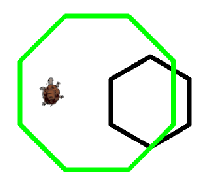
\includegraphics[scale=0.6]{Imagenes/05_Primitivas/relleno1.png}
\end{center}
\vspace{-0.5cm}
y tecleamos:

\texttt{poncolorl\'apiz 1}

\texttt{rellena}

\noindent produce:
\vspace{-0.75cm}
\begin{center}
   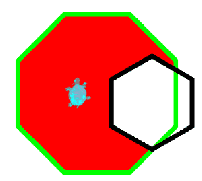
\includegraphics[scale=0.6]{Imagenes/05_Primitivas/relleno2.png}
\end{center}
es decir, ha coloreado de rojo la regi\'on cerrada en la que se encuentra
la tortuga. \\

\noindent Sin embargo, si hacemos:

\texttt{poncolorl\'apiz 0}

\texttt{rellenazona}

\noindent se obtiene:
\begin{center}
   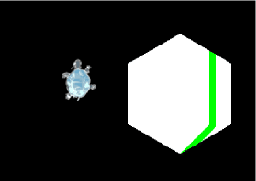
\includegraphics[scale=0.6]{Imagenes/05_Primitivas/relleno3.png}
\end{center}
es decir, rellena todos los p\'ixeles vecinos hasta encontrar una
``frontera'' del color activo.\\

\noindent Este es un buen ejemplo para usar la primitiva \texttt{rellena}:

\noindent \texttt{para mediocirc :c}

\noindent \texttt{\# dibuja un semic\'irculo de diametro :c}
\begin{verbatim}  repite 180 [
    avanza :c * tan 0.5
    giraderecha 1 ]
  avanza :c * tan 0.5
  giraderecha 90 avanza :c
fin

para arcohueco :c
# Utiliza el procedimiento mediocirc para dibujar un arcoiris sin colores
  si :c < 100 [alto]
  mediocirc :c
  giraderecha 180 avanza 20 giraizquierda 90
  arcohueco :c - 40
fin
\end{verbatim}

\noindent \texttt{para arcoiris}

 \texttt{borrapantalla ocultatortuga arcohueco 400}

  \texttt{subel\'apiz giraderecha 90 retrocede 150}

 \texttt{giraizquierda 90 avanza 20 bajal\'apiz}

 \texttt{repitepara [color 0 6]}

 \texttt{ [ poncolorl\'apiz (6-:color) rellena} 

 \verb+  +\texttt{ subel\'apiz giraderecha 90 avanza 20}

 \verb+  +\texttt{ giraizquierda 90 bajal\'apiz ]}

\noindent \texttt{fin}

\begin{center}
   
\includegraphics[scale=0.4]{Imagenes/05_Primitivas/arcoiris.png}
\end{center}
o bien, m\'as realista:

\noindent \texttt{para arcoiris2}

\texttt{borrapantalla ocultatortuga arcohueco 400}

\texttt{subel\'apiz giraderecha 90 retrocede 150}

\texttt{giraizquierda 90 avanza 20 bajal\'apiz}

\texttt{haz \char`\"{}color [ [255 0 0] [255 160 0] [255 255 0] [0 255 0]}

\verb+   + \texttt{ [0 0 255] [75 0 130] [128 0 255] ]}

\texttt{repitepara [colores 1 7]}

\verb+ + \texttt{ [ poncolorl\'apiz elemento :colores :color rellena} 

\verb+  + \texttt{ subel\'apiz giraderecha 90 avanza 20 giraizquierda 90 bajal\'apiz ]}

\noindent \texttt{fin}
\begin{center}
   
\includegraphics[scale=0.6]{Imagenes/05_Primitivas/arcoiris_2.png}
\end{center}

\section{Comandos de ruptura de secuencia}
   \label{Ruptura-Secuencia}
   \index{Ruptura de secuencia}

\textsc{XLogo} tiene tres comandos de ruptura de secuencia: \texttt{alto},
\texttt{detienetodo} y \texttt{devuelve}.

\begin{itemize}
   \item \texttt{alto} \index{alto@\texttt{alto}} puede tener dos
      resultados:
      \begin{itemize}
         \item Si est\'a inclu\'ido en un bucle \texttt{repite}
            \index{repite@\texttt{repite}} o \texttt{mientras},
            \index{mientras@\texttt{mientras}} el programa sale del
            bucle inmediatamente.
         \item Si est\'a en un procedimiento, este es
            terminado.
      \end{itemize}
   \item \texttt{detienetodo} \index{detienetodo@\texttt{detienetodo}}
      interrumpe total y definitivamente todos los procedimientos en
      ejecuci\'on
   \item \texttt{devuelve} \index{devuelve@\texttt{devuelve}}
      (\texttt{dev}) \index{dev@\texttt{dev}} permite salir de un
      procedimiento ``llev\'andose'' un resultado.
\end{itemize}
Al final del manual hay numerosos ejemplos con el uso de estas primitivas.
